% CS.tex
\chapter{Grille Cubed-Sphere}

\section{Définition géométrique de la Cubed-Sphere}

\subsection{La sphère $\mathbb{S}_a^2$}

On note $\mathbb{S}_a^2$ \textit{la sphère} de centre $\mathbf{O} (0,0,0) \in \mathbb{R}^3$ et de rayon $a>0$ :

\begin{equation}
\mathbb{S}_a^2 := \left\lbrace
\mathbf{x} (x,y,z) \in \mathbb{R}^3 / x^2+y^2+z^2 = a^2
\right\rbrace.
\end{equation} 

Un \textit{grand cercle} est un cercle de centre $\mathbf{O}$ et de rayon $a$ tracé sur la sphère $\mathbb{S}_a^2$.
Soit $C$ un grand cercle et $\mathbf{x}_0 \in C$ un point fixé. On choisit l'un des deux sens de parcours le long de $C$ à partir de $\mathbf{x}_0$ et on définit \textit{l'abscisse curviligne} de $\mathbf{x} \in C$ par la distance séparant $\mathbf{x}$ de $\mathbf{x}_0$ le long de $C$. Alors la relation suivante est vérifiée :

\textbf{ICI PREUVE A AJOUTER}

\begin{equation}
\longarc{\mathbf{x}_0  \mathbf{x}} = a \alpha
\end{equation}
où $\alpha \in [ 0, 2 \pi[$ désigne la l'angle $\widehat{\mathbf{x}_0  \mathbf{x}}$ dans le sens choisit (Fig. \ref{fig: grand cercle}). $\alpha$ est \textit{l'angle géodésique} entre $\mathbf{x}_0$ et $\mathbf{x}$.

\begin{figure}[htbp]
\begin{center}
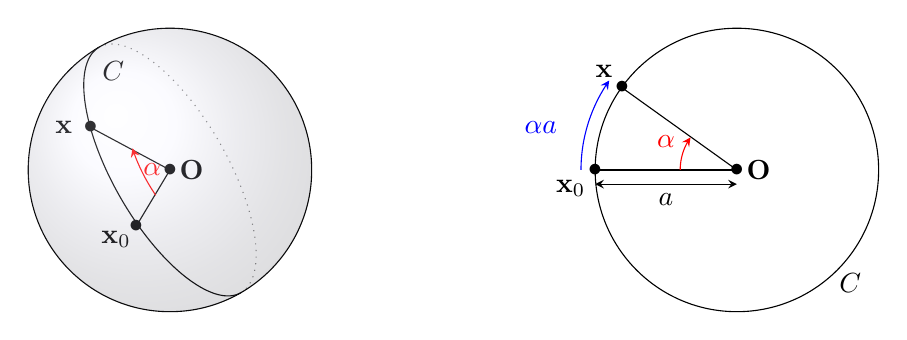
\begin{tikzpicture}[scale=1.8]
	% \draw [color=gray] (-1.5,-1.5) grid[step=0.1] (1.5,1.5); 
	\draw [rotate=-60,samples=100,domain=0:-180] plot({cos(\x)},{0.4*sin(\x)});
	\draw [rotate=-60,samples=100,domain=0:-180,color=gray,dotted] plot({cos(\x)},{-0.4*sin(\x)});
	\draw (-0.4,0.7) node {$C$} ; 
	\draw (-0.24,-0.4) node {$\bullet$} ;
	\draw (-0.38,-0.49) node {$\mathbf{x}_0$} ;
	\draw (0,0) node {$\bullet$} ;
	\draw (0,0) node[right] {$\mathbf{O}$} ;
	\draw (0,0) -- (-0.56,0.3) ;
	\draw (0,0) -- (-0.24,-0.4) ;
	\draw (-0.56,0.3) node {$\bullet$} ;
	\draw (-0.75,0.3) node {$\mathbf{x}$} ;
	\draw [rotate=-60,>=stealth, ->,color=red,domain=-78:-122] plot({0.5*cos(\x)},{0.18*sin(\x)});
	\draw [color=red] (-0.125,0) node {$\alpha$} ;
    \draw (0,0) circle (1cm);
    \shade[ball color=blue!10!white,opacity=0.20] (0,0) circle (1cm);
    
    
    
    
    

    \draw (4,0) circle (1cm);
    \draw (4,0) node {$\bullet$};
    \draw (4,0) node[right] {$\mathbf{O}$};
    \draw (3,0) node {$\bullet$};
    \draw (3,0) node[below left] {$\mathbf{x}_0$};
    \draw (4-.81,.58) node {$\bullet$};
    \draw (4-.81,.58) node[above left] {$\mathbf{x}$};
    \draw (3,0) -- (4,0);
    \draw (4-.81,.58) -- (4,0);
    \draw [>=stealth, <-,color=red,domain=145:180] plot({4+.4*cos(\x)},{.4*sin(\x)});
    \draw (3.5,.2) node[color=red] {$\alpha$};
    \draw [>=stealth, <-,color=blue,domain=145:180] plot({4+1.1*cos(\x)},{1.1*sin(\x)});
    \draw (2.8,.3) node[left, color=blue] {$\alpha a$};
    \draw [>=stealth, <->] (3,-.1) -- (4,-.1);
    \draw (3.5,-.1) node[below] {$a$}; 
    \draw (4.8,-.8) node {$C$};
\end{tikzpicture}
\end{center}
\caption{Un grand cercle sur la sphère $\mathbb{S}_a^2$. L'angle $\alpha$ est tel que $\widehat{\mathbf{x}_0 \mathbf{x}} = \alpha$ et l'abscisse curviligne de $\mathbf{x}$ comptée à partir de $\mathbf{x}_0$ est $a \alpha$.}
\label{fig: grand cercle}
\end{figure}

Soit $\overline{\mathbf{x}} \in \mathbb{S}_a^2$ fixé. Soient $C_1$ et $C_2$ deux grands cercles distincts arbitraires tels que $\overline{\mathbf{x}} \in C_1 \cap C_2$.
Soit $\alpha$ et $\beta$ les abscisses curvilignes le long de $C_1$ et $C_2$, définis à partir de $\mathbf{x}_{1,0} \in C_1$ et $\mathbf{x}_{2,0} \in C_2$ arbitrairement choisis. On définit les vecteurs $\mathbf{e}_{\alpha}(\overline{\mathbf{x}})$ et $\mathbf{e}_{\beta}(\overline{\mathbf{x}})$ (Fig. \ref{fig: e_alpha et e_beta}) par

\begin{equation}
\mathbf{e}_{\alpha}(\overline{\mathbf{x}}) := \dfrac{d \mathbf{x}}{d \alpha}(\overline{\mathbf{x}}) \text{ et } \mathbf{e}_{\beta}(\overline{\mathbf{x}}) := \dfrac{d \mathbf{x}}{d \beta}(\overline{\mathbf{x}})
\end{equation}
$\mathbf{e}_{\alpha}(\overline{\mathbf{x}})$ et $\mathbf{e}_{\beta}(\overline{\mathbf{x}})$ sont tangents aux cercles $C_1$ et $C_2$. $\alpha \rightarrow \mathbf{x}(\alpha)$ (resp.  $\beta \rightarrow \mathbf{x}(\beta)$) désigne le paramétrage du cercle $C_1$ (resp. $C_2$) par l'angle $\alpha$ (resp. $\beta$).

\begin{figure}[htbp]
\begin{center}
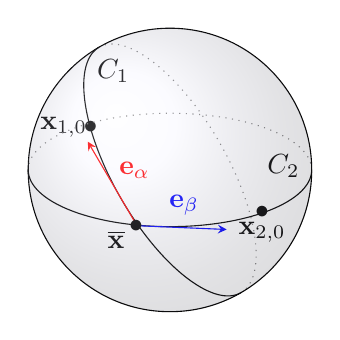
\begin{tikzpicture}[scale=1.8]
	\draw [rotate=-60,samples=100,domain=0:-180] plot({cos(\x)},{0.4*sin(\x)});
	\draw [rotate=-60,samples=100,domain=0:-180,color=gray,dotted] plot({cos(\x)},{-0.4*sin(\x)});
	\draw (-.56,.3) node {$\bullet$} ;
	\draw (-0.75,0.3) node {$\mathbf{x}_{1,0}$} ;
	\draw (-0.4,0.7) node {$C_1$} ; 
	
	\draw [samples=100,domain=0:-180] plot({cos(\x)},{0.4*sin(\x)});
	\draw [samples=100,domain=0:-180,color=gray,dotted] plot({cos(\x)},{-0.4*sin(\x)});
	\draw (0.65,-0.3) node {$\bullet$} ;
	\draw (0.65,-0.3) node[below] {$\mathbf{x}_{2,0}$} ;
	\draw (0.8,0.03) node {$C_2$} ;
	
	\draw [>=stealth, ->, color=blue] (-0.24,-0.393) -- (0.4,-0.42) ;
	\draw [color=blue] (0.1,-0.25) node {$\mathbf{e}_{\beta}$} ;	
	\draw [>=stealth, ->, color=red] (-0.24,-0.38) -- (-0.58,0.20) ;	
	\draw [color=red] (-0.25,0) node {$\mathbf{e}_{\alpha}$} ;
	
	\draw (-0.24,-0.4) node {$\bullet$} ;
	\draw (-0.38,-0.49) node {$\overline{\mathbf{x}}$} ;
	\draw (0,0) circle (1cm);
    \shade[ball color=blue!10!white,opacity=0.20] (0,0) circle (1cm);
\end{tikzpicture}
\end{center}
\caption{Vecteurs $\mathbf{e}_{\alpha}$ et $\mathbf{e}_{\beta}$ associés au cercles $C_1$ et $C_2$ de $\mathbb{S}_a^2$.}
\label{fig: e_alpha et e_beta}
\end{figure}



En tout point $\mathbf{x} \in \mathbb{S}_a^2$, le \textit{plan tangent} $\mathbb{T}_{\mathbf{x}} \mathbb{S}_a^2$ est défini par :

\begin{definition}
On appelle \textit{plan tangent} à la sphère $\mathbb{S}_a^2$ au point $\overline{\mathbf{x}}$ le plan :
\begin{equation}
\mathbb{T}_{\overline{\mathbf{x}}} \mathbb{S}_a^2 := \left\lbrace \mathbf{m} \in \mathbb{R}^3 \ \overrightarrow{\overline{\mathbf{x}} \mathbf{m}} \perp \overrightarrow{O\mathbf{\overline{x}}} \right\rbrace.
\end{equation}
\end{definition}

\begin{proposition}
Soit $\overline{\mathbf{x}} \in \mathbb{S}_a^2$, alors :
\begin{equation}
\mathbf{e}_{\alpha}(\overline{\mathbf{x}})\text{, } \mathbf{e}_{\beta}(\overline{\mathbf{x}}) \in \mathbb{T}_{\overline{\mathbf{x}}} \mathbb{S}_a^2.
\end{equation}
\end{proposition}


\begin{proof}
Soit $\mathbf{x}$ est un point quelconque de $\mathbb{S}_a^2$, donc $\| \mathbf{x} \|^2 = \mathbf{x} \cdot \mathbf{x} = a^2$ est constant.
Alors en dérivant par rapport à $\alpha$, on a :
 
\begin{equation*}
\begin{array}{rcl}
0 & = & \dfrac{d}{d \alpha} ( a^2 )\\
  & = & \dfrac{d}{d \alpha} ( \mathbf{x} \cdot \mathbf{x} )\\
  & = & 2 \mathbf{x} \cdot \dfrac{d \mathbf{x}}{d \alpha}\\
\end{array}
\end{equation*}

En particulier, en $\overline{\mathbf{x}}$, on a :
\begin{equation}
\overline{\mathbf{x}} \cdot \mathbf{e}_{\alpha}(\overline{\mathbf{x}}) = 0
\end{equation}
d'où : $\mathbf{e}_{\alpha}(\overline{\mathbf{x}}) \in \mathbb{T}_{\overline{\mathbf{x}}} \mathbb{S}_a^2$. En dérivant par rapport à $\beta$, on a $\mathbf{e}_{\beta}(\overline{\mathbf{x}}) \in \mathbb{T}_{\overline{\mathbf{x}}} \mathbb{S}_a^2$.
\end{proof}

$\mathbf{e}_{\alpha}(\overline{\mathbf{x}})$ et $\mathbf{e}_{\beta}(\overline{\mathbf{x}})$ sont dans le plan $\mathbb{T}_{\overline{\mathbf{x}}}\mathbb{S}_a^2$. De plus, $C_1 \neq C_2$ donc $\mathbf{e}_{\alpha}(\overline{\mathbf{x}})$ et $\mathbf{e}_{\beta}(\overline{\mathbf{x}})$ ne sont pas colinéaires. On en déduit que $\mathbf{e}_{\alpha}(\overline{\mathbf{x}})$ et $\mathbf{e}_{\beta}(\overline{\mathbf{x}})$ engendrent $\mathbb{T}_{\overline{\mathbf{x}}} \mathbb{S}_a^2$. En général, $\mathbf{e}_{\alpha}(\overline{\mathbf{x}})$ et $\mathbf{e}_{\beta}(\overline{\mathbf{x}})$ ne sont pas orthogonaux.

\begin{definition}
On définit $(\mathbf{e}^{\alpha}(\overline{\mathbf{x}}), \mathbf{e}^{\beta}(\overline{\mathbf{x}}))$ la \textit{base duale} de $(\mathbf{e}_{\alpha}(\overline{\mathbf{x}}), \mathbf{e}_{\beta}(\overline{\mathbf{x}}))$.
Les vecteurs $\mathbf{e}^{\alpha}(\overline{\mathbf{x}})$ et $\mathbf{e}^{\beta}(\overline{\mathbf{x}})$ sont les vecteurs de $\mathbb{T}_{\overline{\mathbf{x}}}\mathbb{S}_a^2$ vérifiant :

\begin{equation}
\left\lbrace
\begin{array}{rcccl}
\mathbf{e}_{\alpha}(\overline{\mathbf{x}}) \cdot \mathbf{e}^{\alpha}(\overline{\mathbf{x}}) & = & 1 & = & \mathbf{e}_{\beta}(\overline{\mathbf{x}}) \cdot \mathbf{e}^{\beta}(\overline{\mathbf{x}}) \\
\mathbf{e}_{\alpha}(\overline{\mathbf{x}}) \cdot \mathbf{e}^{\beta}(\overline{\mathbf{x}}) & = & 0 & = & \mathbf{e}_{\beta}(\overline{\mathbf{x}}) \cdot \mathbf{e}^{\alpha}(\overline{\mathbf{x}}) \\
\end{array}
\right.
\label{eq: dualite alpha beta}
\end{equation}

\end{definition}

\begin{proposition}
$(\mathbf{e}^{\alpha}(\overline{\mathbf{x}}), \mathbf{e}^{\beta}(\overline{\mathbf{x}}))$ la base duale de $(\mathbf{e}_{\alpha}(\overline{\mathbf{x}}), \mathbf{e}_{\beta}(\overline{\mathbf{x}}))$ est définie de façon unique.
\end{proposition}

\begin{proof}
Il suffit de remarquer que
\begin{equation}
\begin{bmatrix}
\mathbf{e}_{\alpha}(\overline{\mathbf{x}}) , \mathbf{e}_{\beta}(\overline{\mathbf{x}})
\end{bmatrix}^T \cdot 
\begin{bmatrix}
\mathbf{e}^{\alpha}(\overline{\mathbf{x}}) , \mathbf{e}^{\beta}(\overline{\mathbf{x}})
\end{bmatrix} = Id
\end{equation}
Alors 
\begin{equation}
\begin{bmatrix}
\mathbf{e}^{\alpha}(\overline{\mathbf{x}}) , \mathbf{e}^{\beta}(\overline{\mathbf{x}})
\end{bmatrix} = 
\begin{bmatrix}
\mathbf{e}_{\alpha}(\overline{\mathbf{x}}) , \mathbf{e}_{\beta}(\overline{\mathbf{x}})
\end{bmatrix}^{-T}.
\end{equation}
\end{proof}

A partir de ces différentes bases, le \textit{gradient} est donné par

\begin{proposition}
Soit $h : \mathbb{S}_a^2 \mapsto \mathbb{R}$ une fonction régulière, le gradient de $h$, $\nabla_T h(\mathbf{x}) \in \mathbb{T}_{\mathbf{x}}\mathbb{S}^2_a$, est

\begin{equation}
\nabla_{T} h(\overline{\mathbf{x}}) := \dfrac{\partial}{\partial \alpha} \left( h(\overline{\mathbf{x}}) \right)_{| \mathbf{x} \in C_1} \mathbf{e}^{\alpha}(\overline{\mathbf{x}}) + \dfrac{\partial}{\partial \beta}\left(  h(\overline{\mathbf{x}}) \right)_{| \mathbf{x} \in C_2} \mathbf{e}^{\beta}(\overline{\mathbf{x}}).
\label{eq: gradient}
\end{equation}
\end{proposition}

Pour alléger les notations, nous noterons abusivement les quantités $h$, $\mathbf{e}_{\alpha}$, $\mathbf{e}^{\beta}$ ... au lieu de $h(\mathbf{x})$, $\mathbf{e}_{\alpha}(\mathbf{x})$, $\mathbf{e}^{\beta}(\mathbf{x})$, ...


\begin{proposition}
Soit $u: \mathbb{R}^3 \mapsto \mathbb{R}$ et $\mathbf{x} \in \mathbb{R}^3$. On pose $\hat{u} : = u_{|\mathbb{S}_a^2}$ la restriction de $u$ à la sphère $\mathbb{S}_a^2$. Alors $\nabla_{T} \hat{u} (\mathbf{x})$ est la projection orthogonale de $\nabla_{\mathbb{R}^3} u (\mathbf{x})$ sur le plan tangent $\mathbb{T}_{\mathbf{x}} \mathbb{S}_a^2$.

\begin{equation}
\nabla_T \hat{u} = \nabla_{\mathbb{R}^3} u - \mathbf{n} \left( \mathbf{n} \cdot \nabla_{\mathbb{R}^3} u \right)
\end{equation}

avec $\mathbf{n}$ la normale unitaire extérieure.
\label{prop:gradient_project}
\end{proposition}

\begin{proof}
Pour montrer cette égalité, on montre que les deux termes sont égaux dans trois directions distinctes. on pose $\mathbf{n}$ la normale unitaire extérieure à la sphère $\mathbb{S}_a^2$.
\begin{itemize}
\item Direction $\mathbf{e}_{\alpha}$ :
d'une part on a :
\begin{equation}
\nabla_T \hat{u} \cdot \mathbf{e}_{\alpha} = \dfrac{\partial \hat{u}}{\partial \alpha}_{| \mathbf{x} \in C_1}= \dfrac{\partial u}{\partial \alpha}_{| \mathbf{x} \in C_1}.
\end{equation}
D'autres part, on a :
\begin{equation}
\left( \nabla_{\mathbb{R}^3} u - \mathbf{n} \left( \mathbf{n} \cdot \nabla_{\mathbb{R}^3} u \right) \right) \cdot \mathbf{e}_{\alpha} = \nabla_{\mathbb{R}^3} u \cdot \mathbf{e}_{\alpha}
\end{equation}
car $\mathbf{n}$ est normal à la sphère donc $\mathbf{n}$ est normal à $\mathbf{e}_{\alpha}$.
Or :
\begin{equation}
\nabla_{\mathbb{R}^3} u \cdot \mathbf{e}_{\alpha} = \dfrac{\partial u}{\partial \alpha}_{| \mathbf{x} \in C_1} = \nabla_T \hat{u} \cdot \mathbf{e}_{\alpha}.
\end{equation}

\item Dans la direction $\mathbf{e}_{\beta}$, on a de la même manière :
\begin{equation}
\nabla_{\mathbb{R}^3} u \cdot \mathbf{e}_{\beta} = \nabla_T \hat{u} \cdot \mathbf{e}_{\beta}.
\end{equation}

\item Dans la direction $\mathbf{n}$ on a d'une part :
\begin{equation}
\nabla_T \hat{u} \cdot \mathbf{n} = 0 
\end{equation}
car $\nabla_T \hat{u}$ est tangent à la sphère. D'autres part :
\begin{equation}
\left( \nabla_{\mathbb{R}^3} u - \mathbf{n} \left( \mathbf{n} \cdot \nabla_{\mathbb{R}^3} u \right) \right) \cdot \mathbf{n} = \nabla_{\mathbb{R}^3} u \cdot \mathbf{n}- \mathbf{n} \cdot \nabla_{\mathbb{R}^3} u = 0
\end{equation}
\end{itemize}
$(\mathbf{e}_{\alpha}, \mathbf{e}_{\beta}, \mathbf{n})$ est une base de $\mathbb{R}^3$, d'où l'égalité souhaitée.
\end{proof}




















\subsection{Définition de la Cubed-Sphere}

Définissons la Cubed-Sphere associée à la base orthonormée $(\mathbf{i}, \mathbf{j}, \mathbf{k})$ de $\mathbb{R}^3$.
On définit les points suivants (Voir Figure \ref{fig: sphere NSEWFB}) sur la sphère $\mathbb{S}_a^2$ :
\begin{itemize}
\item $\mathbf{N}$ le point de coordonnées dans $\mathbb{R}^3$ : $(0,0,a)$,
\item $\mathbf{S}$ le point de coordonnées $(0,0,-a)$,
\item $\mathbf{E}$ le point de coordonnées $(0,a,0)$,
\item $\mathbf{W}$ le point de coordonnées $(0,-a,0)$,
\item $\mathbf{F}$ le point de coordonnées $(a,0,0)$,
\item $\mathbf{B}$ le point de coordonnées $(-a,0,0)$.
\end{itemize}


\begin{figure}[htbp]
\begin{center}
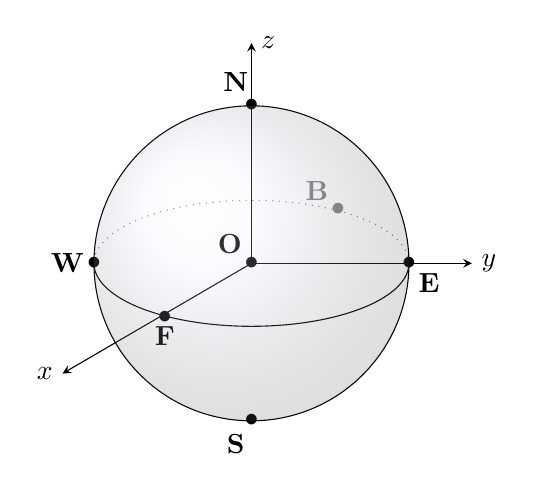
\begin{tikzpicture}[scale=2]
	\draw [samples=100,domain=-180:0] plot({cos(\x)},{0.4*sin(\x)});
	\draw [dotted, color=black!50, samples=100,domain=0:180] plot({cos(\x)},{0.4*sin(\x)});

	\draw  (0,0) node {$\bullet$} ;
	\draw  (0,0) node[above left] {$\mathbf{O}$} ;
	\draw  (0,1) node {$\bullet$} ;
	\draw  (-0.1,1.15) node {$\mathbf{N}$} ;
	\draw  (0,-1) node {$\bullet$} ;
	\draw  (-0.1,-1.15) node {$\mathbf{S}$} ;
	\draw  (1,0) node {$\bullet$} ;
	\draw  (1,0) node[below right] {$\mathbf{E}$} ;
	\draw  (-1,0) node {$\bullet$} ;
	\draw  (-1,0) node[left] {$\mathbf{W}$} ;	
	\draw  (-0.55,-0.34) node {$\bullet$} ;
	\draw  (-0.55,-0.34) node[below] {$\mathbf{F}$} ;	
	\draw  (0.55,0.34) node[color=black!50] {$\bullet$} ;
	\draw  (0.55,0.34) node[color=black!50, above left] {$\mathbf{B}$} ;	
	
	\draw [>=stealth, ->] (0,0) -- (-1.2,-0.7) ;
	\draw  (-1.2,-0.7) node[left] {$x$} ;
	\draw [>=stealth, ->] (0,0) -- (0,1.4) ;
	\draw  (0,1.4) node[right] {$z$} ;
	\draw [>=stealth, ->] (0,0) -- (1.4,0) ;
	\draw  (1.4,0) node[right] {$y$} ;
	\draw (0,0) circle (1cm);
    \shade[ball color=blue!10!white,opacity=0.20] (0,0) circle (1cm);
\end{tikzpicture}
\end{center}
\caption{Sphère $\mathbb{S}_a^2$ avec les 6 points $\mathbf{N}$ (Nord), $\mathbf{S}$ (Sud), $\mathbf{E}$ (Est), $\mathbf{W}$ (Ouest), $\mathbf{F}$ (Avant) et $\mathbf{B}$ (Arrière).}
\label{fig: sphere NSEWFB}
\end{figure}

Un grand cercle est l'intersection de la sphère $\mathbb{S}_a^2$ avec un plan contenant le point $\mathbf{O}$. On définit les grands cercles suivants (Fig \ref{fig: grands cercles panel I}) :

\begin{itemize}
\item $C_V^1 = \Vect(\mathbf{i}-\mathbf{j}, \mathbf{k}) \cap \mathbb{S}_a^2$,
\item $C_V^2 = \Vect(\mathbf{i}+\mathbf{j}, \mathbf{k}) \cap \mathbb{S}_a^2$, il s'agit d'une rotation de $C_V^1$ d'un angle de $\pi/2$ autour de $(Oz)$,
\item $C_{II}^1 = \Vect(\mathbf{i}+\mathbf{k}, \mathbf{j}) \cap \mathbb{S}_a^2$, $C_{II}^2$ est une rotation de $C_{II}^1$ d'un angle de $\pi/2$ autour de $(Oy)$,
\item $C_{II}^2 = \Vect(\mathbf{i}-\mathbf{k}, \mathbf{j}) \cap \mathbb{S}_a^2$,
\item $C_I^1=\Vect(\mathbf{j}-\mathbf{k},\mathbf{i}) \cap \mathbb{S}_a^2$,
\item $C_I^2=\Vect(\mathbf{j}+\mathbf{k},\mathbf{i}) \cap \mathbb{S}_a^2$, $C_I^2$ est une rotation de $C_I^1$ autour de $(Ox)$ d'un angle de $\pi/2$
\end{itemize}

\begin{figure}[htbp]
\begin{center}
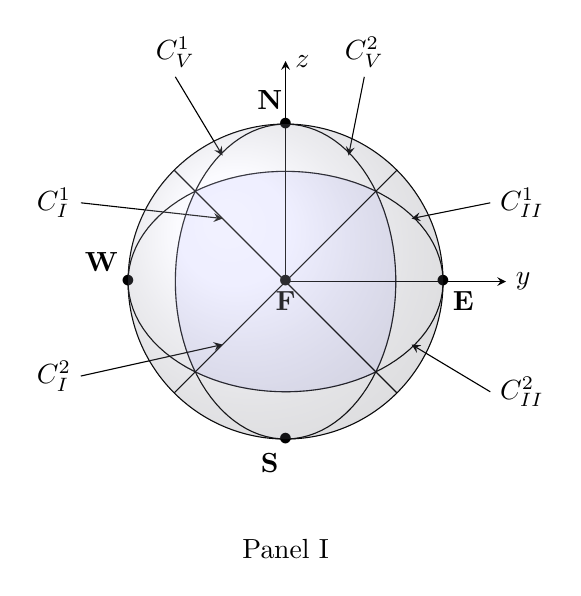
\begin{tikzpicture}[scale=2]
	%\draw [color=gray] (-1.5,-1.5) grid[step=0.1] (1.5,1.5);
	\draw [samples=100,domain=-180:180] plot({cos(\x)},{0.7*sin(\x)});
	\draw [samples=100,domain=180:-180] plot({0.7*cos(\x)},{sin(\x)}); 
	
	\filldraw[draw=black,fill=blue!30!white,opacity=0.20]
	plot [smooth,domain=-35:35] ({0.7*cos(\x)},{sin(\x)})
	-- plot [smooth,domain=55:125] ({cos(\x)},{0.7*sin(\x)})
	-- plot [smooth,domain=140:215] ({0.7*cos(\x)},{sin(\x)})
	-- plot [smooth,domain=230:305] ({cos(\x)},{0.7*sin(\x)})
	-- cycle;
	
	\draw (-0.707,0.707) -- (0.707,-0.707) ;
	\draw [>=stealth, <-] (-0.4,0.4) -- (-1.3,0.5) ;
	\draw  (-1.3,0.5) node[left] {$C_I^1$} ;
	\draw (-0.707,-0.707) -- (0.707,0.707) ;
	\draw [>=stealth, <-] (-0.4,-0.4) -- (-1.3,-0.6) ;
	\draw  (-1.3,-0.6) node[left] {$C_I^2$} ;
	
	\draw [>=stealth, ->] (0.5,1.3) -- (0.4,0.8) ;
	\draw  (0.5,1.3) node[above] {$C_V^2$} ;
	\draw [>=stealth, ->] (-0.7,1.3) -- (-0.4,0.8) ;
	\draw  (-0.7,1.3) node[above] {$C_V^1$} ;
	\draw [>=stealth, ->] (1.3,0.5) -- (0.8,0.4) ;
	\draw  (1.3,0.5) node[right] {$C_{II}^1$} ;
	\draw [>=stealth, ->] (1.3,-0.7) -- (0.8,-0.4) ;
	\draw  (1.3,-0.7) node[right] {$C_{II}^2$} ;
	
	\draw [>=stealth, ->] (0,0) -- (0,1.4) ;
	\draw  (0,1.4) node[right] {$z$} ;
	\draw [>=stealth, ->] (0,0) -- (1.4,0) ;
	\draw  (1.4,0) node[right] {$y$} ;
	
	\draw  (0,1) node {$\bullet$} ;
	\draw  (-0.1,1.15) node {$\mathbf{N}$} ;
	\draw  (0,-1) node {$\bullet$} ;
	\draw  (-0.1,-1.15) node {$\mathbf{S}$} ;
	\draw  (1,0) node {$\bullet$} ;
	\draw  (1,0) node[below right] {$\mathbf{E}$} ;
	\draw  (-1,0) node {$\bullet$} ;
	\draw  (-1,0) node[above left] {$\mathbf{W}$} ;
	\draw  (0,0) node {$\bullet$} ;
	\draw  (0,0) node[below] {$\mathbf{F}$} ;
	
	\draw  (0,-1.7) node {Panel I} ;

	\draw (0,0) circle (1cm);
    \shade[ball color=blue!10!white,opacity=0.20] (0,0) circle (1cm);

\end{tikzpicture}
\caption{Grands cercles visibles sur le Panel I de la sphère $\mathbb{S}_a^2$.}
\end{center}
\label{fig: grands cercles panel I}
\end{figure}

La construction de la Cubed-Sphere fait intervenir six zones recouvrant la sphère $\mathbb{S}_a^2$ appelés \textit{panels}. Chaque panel est délimité par quatre grands cercles (Fig. \ref{fig: panel I to VI}).

\begin{definition}
\begin{itemize}
\item  \textbf{Panels I et III : }Les panels I et III sont définis par les points de $\mathbb{S}_a^2$ délimités par les grands cercles $C_V^1$, $C_V^2$, $C_{II}^1$ et $C_{II}^2$. Le panel III est le symétrique du panel I par la symétrie ponctuelle de centre $\mathbf{O}$.Le panel I ne contient que des points $(x,y,z)$ tels que $x>0$, le panel III ne contient que des points tels que $x<0$.
\item \textbf{Panels II et IV : }Les panels II et IV sont définis par les points de $\mathbb{S}_a^2$ délimités par les grands cercles $C_V^1$, $C_V^2$, $C_{I}^1$ et $C_{I}^2$. Le panel IV est le symétrique du panel II par la symétrie ponctuelle de centre $\mathbf{O}$. Le panel II ne contient que des points $(x,y,z)$ tels que $y>0$, le panel IV ne contient que des points tels que $y<0$.
\item \textbf{Panels V et VI : }Les panels V et VI sont définis par les points de $\mathbb{S}_a^2$ délimités par les grands cercles $C_I^1$, $C_I^2$, $C_{II}^1$ et $C_{II}^2$. Le panel VI est le symétrique du panel V par la symétrie ponctuelle de centre $\mathbf{O}$. Le panel V ne contient que des points $(x,y,z)$ tels que $z>0$, le panel VI ne contient que des points tels que $z<0$.
\end{itemize}
\end{definition}






\begin{figure}[htbp]
\begin{center}
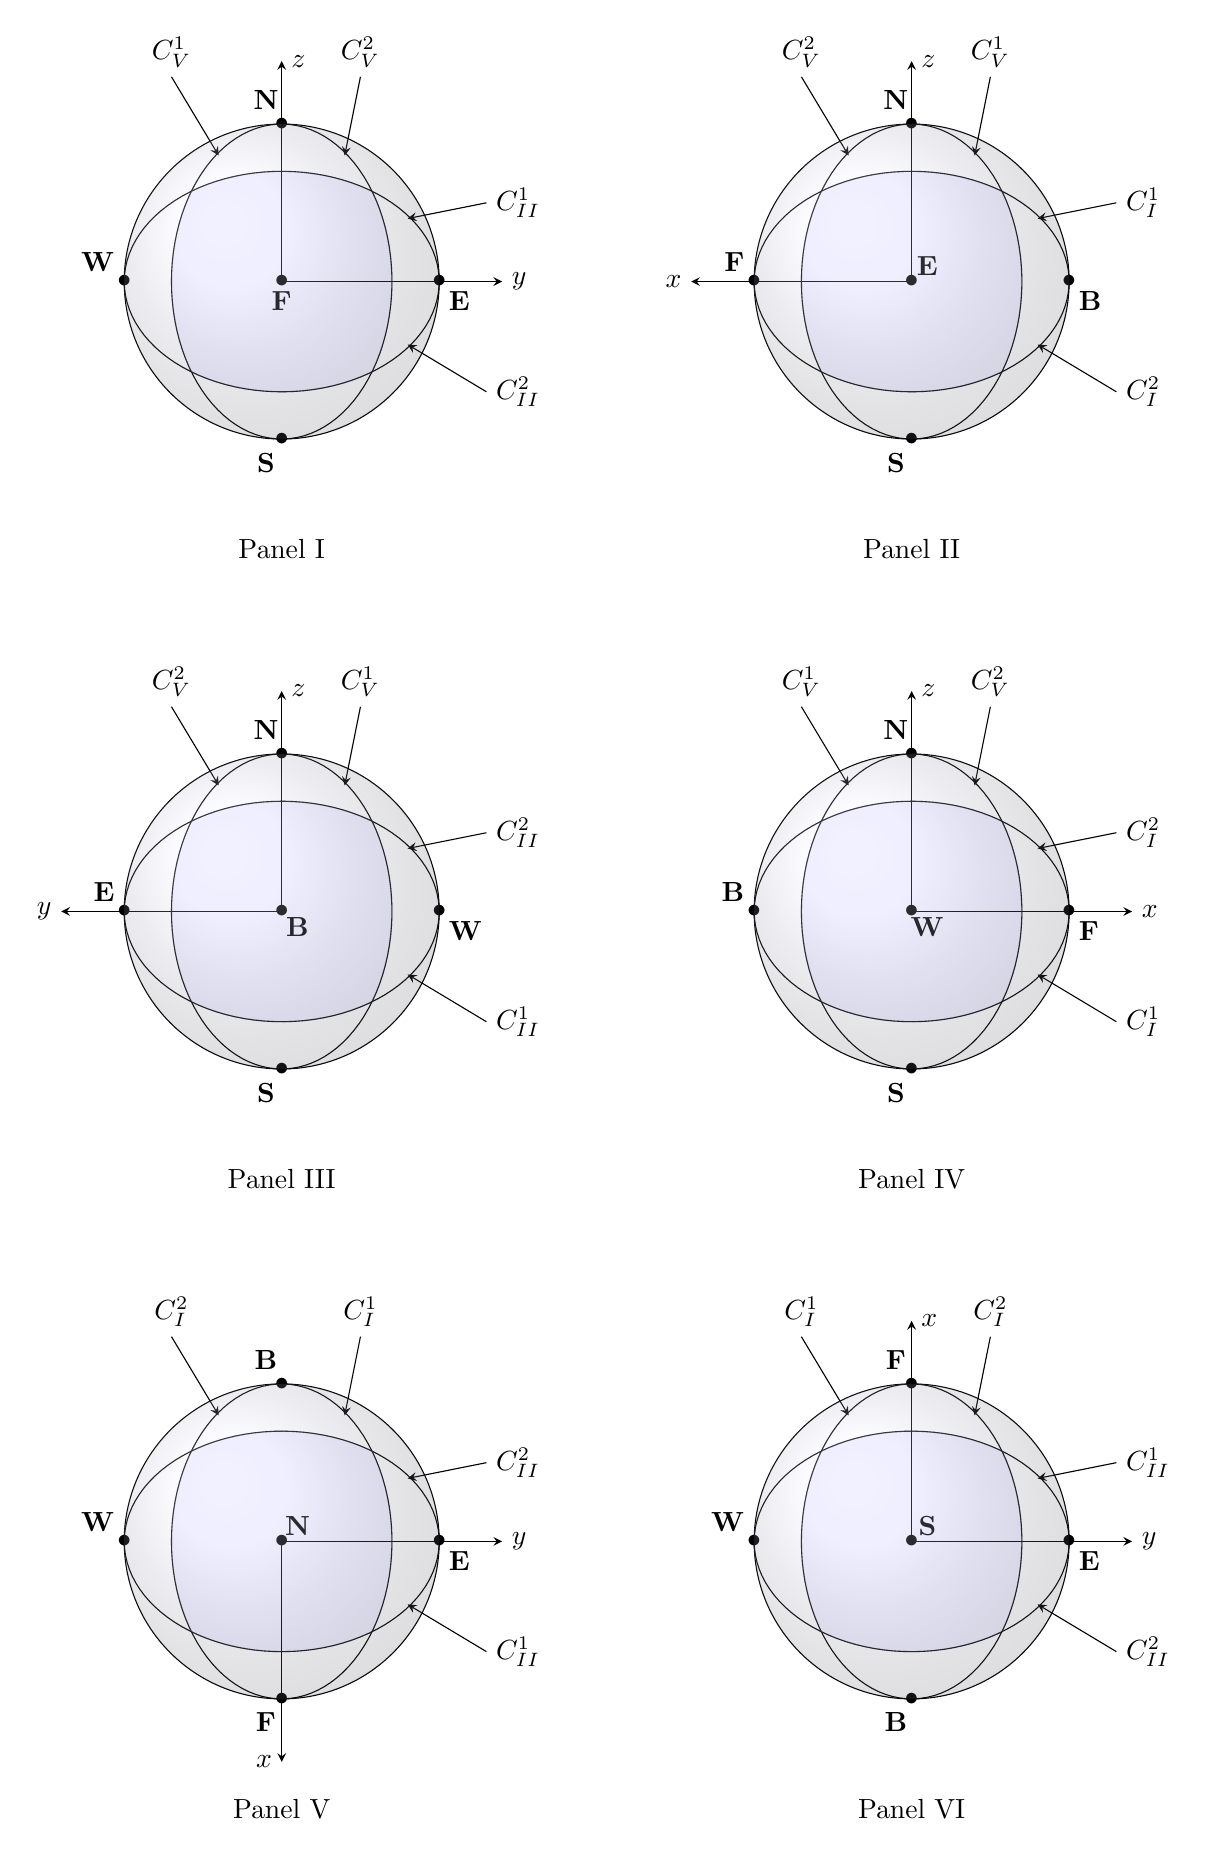
\begin{tikzpicture}[scale=2]
	%\draw [color=gray] (-1.5,-1.5) grid[step=0.1] (1.5,1.5);
	\draw [samples=100,domain=-180:180] plot({cos(\x)},{0.7*sin(\x)});
	\draw [samples=100,domain=180:-180] plot({0.7*cos(\x)},{sin(\x)}); 
	
	\filldraw[draw=black,fill=blue!30!white,opacity=0.20]
	plot [smooth,domain=-35:35] ({0.7*cos(\x)},{sin(\x)})
	-- plot [smooth,domain=55:125] ({cos(\x)},{0.7*sin(\x)})
	-- plot [smooth,domain=140:215] ({0.7*cos(\x)},{sin(\x)})
	-- plot [smooth,domain=230:305] ({cos(\x)},{0.7*sin(\x)})
	-- cycle;
	
	\draw [>=stealth, ->] (0.5,1.3) -- (0.4,0.8) ;
	\draw  (0.5,1.3) node[above] {$C_V^2$} ;
	\draw [>=stealth, ->] (-0.7,1.3) -- (-0.4,0.8) ;
	\draw  (-0.7,1.3) node[above] {$C_V^1$} ;
	\draw [>=stealth, ->] (1.3,0.5) -- (0.8,0.4) ;
	\draw  (1.3,0.5) node[right] {$C_{II}^1$} ;
	\draw [>=stealth, ->] (1.3,-0.7) -- (0.8,-0.4) ;
	\draw  (1.3,-0.7) node[right] {$C_{II}^2$} ;
	
	\draw [>=stealth, ->] (0,0) -- (0,1.4) ;
	\draw  (0,1.4) node[right] {$z$} ;
	\draw [>=stealth, ->] (0,0) -- (1.4,0) ;
	\draw  (1.4,0) node[right] {$y$} ;
	
	\draw  (0,1) node {$\bullet$} ;
	\draw  (-0.1,1.15) node {$\mathbf{N}$} ;
	\draw  (0,-1) node {$\bullet$} ;
	\draw  (-0.1,-1.15) node {$\mathbf{S}$} ;
	\draw  (1,0) node {$\bullet$} ;
	\draw  (1,0) node[below right] {$\mathbf{E}$} ;
	\draw  (-1,0) node {$\bullet$} ;
	\draw  (-1,0) node[above left] {$\mathbf{W}$} ;
	\draw  (0,0) node {$\bullet$} ;
	\draw  (0,0) node[below] {$\mathbf{F}$} ;
	
	\draw  (0,-1.7) node {Panel I} ;

	\draw (0,0) circle (1cm);
    \shade[ball color=blue!10!white,opacity=0.20] (0,0) circle (1cm);




	\draw [samples=100,domain=-180:180] plot({4+cos(\x)},{0.7*sin(\x)});
	\draw [samples=100,domain=180:-180] plot({4+0.7*cos(\x)},{sin(\x)}); 
	
	\filldraw[draw=black,fill=blue!30!white,opacity=0.20]
	plot [smooth,domain=-35:35] ({4+0.7*cos(\x)},{sin(\x)})
	-- plot [smooth,domain=55:125] ({4+cos(\x)},{0.7*sin(\x)})
	-- plot [smooth,domain=140:215] ({4+0.7*cos(\x)},{sin(\x)})
	-- plot [smooth,domain=230:305] ({4+cos(\x)},{0.7*sin(\x)})
	-- cycle;
	
	\draw [>=stealth, ->] (4.5,1.3) -- (4.4,0.8) ;
	\draw  (4.5,1.3) node[above] {$C_V^1$} ;
	\draw [>=stealth, ->] (3.3,1.3) -- (3.6,0.8) ;
	\draw  (3.3,1.3) node[above] {$C_V^2$} ;
	\draw [>=stealth, ->] (5.3,0.5) -- (4.8,0.4) ;
	\draw  (5.3,0.5) node[right] {$C_{I}^1$} ;
	\draw [>=stealth, ->] (5.3,-0.7) -- (4.8,-0.4) ;
	\draw  (5.3,-0.7) node[right] {$C_{I}^2$} ;
	
	\draw [>=stealth, ->] (4,0) -- (4,1.4) ;
	\draw  (4,1.4) node[right] {$z$} ;
	\draw [>=stealth, ->] (4,0) -- (4-1.4,0) ;
	\draw  (4-1.4,0) node[left] {$x$} ;
	
	\draw  (4,1) node {$\bullet$} ;
	\draw  (4-0.1,1.15) node {$\mathbf{N}$} ;
	\draw  (4,-1) node {$\bullet$} ;
	\draw  (4-0.1,-1.15) node {$\mathbf{S}$} ;
	\draw  (5,0) node {$\bullet$} ;
	\draw  (5,0) node[below right] {$\mathbf{B}$} ;
	\draw  (4-1,0) node {$\bullet$} ;
	\draw  (4-1,0) node[above left] {$\mathbf{F}$} ;
	\draw  (4,0) node {$\bullet$} ;
	\draw  (4.1,0.1) node {$\mathbf{E}$} ;
	
	\draw  (4,-1.7) node {Panel II} ;

	\draw (4,0) circle (1cm);
    \shade[ball color=blue!10!white,opacity=0.20] (4,0) circle (1cm);






	\draw [samples=100,domain=-180:180] plot({cos(\x)},{-4+0.7*sin(\x)});
	\draw [samples=100,domain=180:-180] plot({0.7*cos(\x)},{-4+sin(\x)}); 
	
	\filldraw[draw=black,fill=blue!30!white,opacity=0.20]
	plot [smooth,domain=-35:35] ({0.7*cos(\x)},{-4+sin(\x)})
	-- plot [smooth,domain=55:125] ({cos(\x)},{-4+0.7*sin(\x)})
	-- plot [smooth,domain=140:215] ({0.7*cos(\x)},{-4+sin(\x)})
	-- plot [smooth,domain=230:305] ({cos(\x)},{-4+0.7*sin(\x)})
	-- cycle;
	
	\draw [>=stealth, ->] (0.5,-4+1.3) -- (0.4,-4+0.8) ;
	\draw  (0.5,-4+1.3) node[above] {$C_V^1$} ;
	\draw [>=stealth, ->] (-0.7,-4+1.3) -- (-0.4,-4+0.8) ;
	\draw  (-0.7,-4+1.3) node[above] {$C_V^2$} ;
	\draw [>=stealth, ->] (1.3,-4+0.5) -- (0.8,-4+0.4) ;
	\draw  (1.3,-4+0.5) node[right] {$C_{II}^2$} ;
	\draw [>=stealth, ->] (1.3,-4-0.7) -- (0.8,-4-0.4) ;
	\draw  (1.3,-4-0.7) node[right] {$C_{II}^1$} ;
	
	\draw [>=stealth, ->] (0,-4) -- (0,-4+1.4) ;
	\draw  (0,-4+1.4) node[right] {$z$} ;
	\draw [>=stealth, ->] (0,-4) -- (-1.4,-4) ;
	\draw  (-1.4,-4) node[left] {$y$} ;
	
	\draw  (0,-4+1) node {$\bullet$} ;
	\draw  (-0.1,-4+1.15) node {$\mathbf{N}$} ;
	\draw  (0,-4-1) node {$\bullet$} ;
	\draw  (-0.1,-4-1.15) node {$\mathbf{S}$} ;
	\draw  (1,-4) node {$\bullet$} ;
	\draw  (1,-4) node[below right] {$\mathbf{W}$} ;
	\draw  (-1,-4) node {$\bullet$} ;
	\draw  (-1,-4) node[above left] {$\mathbf{E}$} ;
	\draw  (0,-4) node {$\bullet$} ;
	\draw  (0.1,-4.1) node {$\mathbf{B}$} ;
	
	\draw  (0,-4-1.7) node {Panel III} ;

	\draw (0,-4) circle (1cm);
    \shade[ball color=blue!10!white,opacity=0.20] (0,-4) circle (1cm);




	\draw [samples=100,domain=-180:180] plot({4+cos(\x)},{-4+0.7*sin(\x)});
	\draw [samples=100,domain=180:-180] plot({4+0.7*cos(\x)},{-4+sin(\x)}); 
	
	\filldraw[draw=black,fill=blue!30!white,opacity=0.20]
	plot [smooth,domain=-35:35] ({4+0.7*cos(\x)},{-4+sin(\x)})
	-- plot [smooth,domain=55:125] ({4+cos(\x)},{-4+0.7*sin(\x)})
	-- plot [smooth,domain=140:215] ({4+0.7*cos(\x)},{-4+sin(\x)})
	-- plot [smooth,domain=230:305] ({4+cos(\x)},{-4+0.7*sin(\x)})
	-- cycle;
	
	\draw [>=stealth, ->] (4+0.5,-4+1.3) -- (4+0.4,-4+0.8) ;
	\draw  (4+0.5,-4+1.3) node[above] {$C_V^2$} ;
	\draw [>=stealth, ->] (4-0.7,-4+1.3) -- (4-0.4,-4+.8) ;
	\draw  (4-0.7,-4+1.3) node[above] {$C_V^1$} ;
	\draw [>=stealth, ->] (4+1.3,-4+0.5) -- (4+0.8,-4+0.4) ;
	\draw  (4+1.3,-4+.5) node[right] {$C_{I}^2$} ;
	\draw [>=stealth, ->] (4+1.3,-4-0.7) -- (4+0.8,-4-0.4) ;
	\draw  (4+1.3,-4-0.7) node[right] {$C_{I}^1$} ;
	
	\draw [>=stealth, ->] (4,-4) -- (4,-4+1.4) ;
	\draw  (4,-4+1.4) node[right] {$z$} ;
	\draw [>=stealth, ->] (4,-4) -- (5.4,-4) ;
	\draw  (5.4,-4) node[right] {$x$} ;
	
	\draw  (4,-4+1) node {$\bullet$} ;
	\draw  (4-0.1,-4+1.15) node {$\mathbf{N}$} ;
	\draw  (4,-4-1) node {$\bullet$} ;
	\draw  (4-0.1,-4-1.15) node {$\mathbf{S}$} ;
	\draw  (5,-4) node {$\bullet$} ;
	\draw  (5,-4) node[below right] {$\mathbf{F}$} ;
	\draw  (4-1,-4) node {$\bullet$} ;
	\draw  (4-1,-4) node[above left] {$\mathbf{B}$} ;
	\draw  (4,-4) node {$\bullet$} ;
	\draw  (4.1,-4.1) node {$\mathbf{W}$} ;
	
	\draw  (4,-4-1.7) node {Panel IV} ;

	\draw (4,-4) circle (1cm);
    \shade[ball color=blue!10!white,opacity=0.20] (4,-4) circle (1cm);




	\draw [samples=100,domain=-180:180] plot({cos(\x)},{-8+0.7*sin(\x)});
	\draw [samples=100,domain=180:-180] plot({0.7*cos(\x)},{-8+sin(\x)}); 
	
	\filldraw[draw=black,fill=blue!30!white,opacity=0.20]
	plot [smooth,domain=-35:35] ({0.7*cos(\x)},{-8+sin(\x)})
	-- plot [smooth,domain=55:125] ({cos(\x)},{0.7*sin(\x)-8})
	-- plot [smooth,domain=140:215] ({0.7*cos(\x)},{sin(\x)-8})
	-- plot [smooth,domain=230:305] ({cos(\x)},{0.7*sin(\x)-8})
	-- cycle;
	
	\draw [>=stealth, ->] (0.5,1.3-8) -- (0.4,0.8-8) ;
	\draw  (0.5,1.3-8) node[above] {$C_I^1$} ;
	\draw [>=stealth, ->] (-0.7,1.3-8) -- (-0.4,0.8-8) ;
	\draw  (-0.7,1.3-8) node[above] {$C_I^2$} ;
	\draw [>=stealth, ->] (1.3,0.5-8) -- (0.8,0.4-8) ;
	\draw  (1.3,0.5-8) node[right] {$C_{II}^2$} ;
	\draw [>=stealth, ->] (1.3,-0.7-8) -- (0.8,-0.4-8) ;
	\draw  (1.3,-0.7-8) node[right] {$C_{II}^1$} ;
	
	\draw [>=stealth, ->] (0,0-8) -- (0,-1.4-8) ;
	\draw  (0,-1.4-8) node[left] {$x$} ;
	\draw [>=stealth, ->] (0,0-8) -- (1.4,0-8) ;
	\draw  (1.4,0-8) node[right] {$y$} ;
	
	\draw  (0,1-8) node {$\bullet$} ;
	\draw  (-0.1,1.15-8) node {$\mathbf{B}$} ;
	\draw  (0,-1-8) node {$\bullet$} ;
	\draw  (-0.1,-1.15-8) node {$\mathbf{F}$} ;
	\draw  (1,0-8) node {$\bullet$} ;
	\draw  (1,0-8) node[below right] {$\mathbf{E}$} ;
	\draw  (-1,0-8) node {$\bullet$} ;
	\draw  (-1,0-8) node[above left] {$\mathbf{W}$} ;
	\draw  (0,0-8) node {$\bullet$} ;
	\draw  (0.1,0.1-8) node {$\mathbf{N}$} ;
	
	\draw  (0,-1.7-8) node {Panel V} ;

	\draw (0,0-8) circle (1cm);
    \shade[ball color=blue!10!white,opacity=0.20] (0,0-8) circle (1cm);



	\draw [samples=100,domain=-180:180] plot({4+cos(\x)},{0.7*sin(\x)-8});
	\draw [samples=100,domain=180:-180] plot({4+0.7*cos(\x)},{sin(\x)-8}); 
	
	\filldraw[draw=black,fill=blue!30!white,opacity=0.20]
	plot [smooth,domain=-35:35] ({4+0.7*cos(\x)},{sin(\x)-8})
	-- plot [smooth,domain=55:125] ({4+cos(\x)},{0.7*sin(\x)-8})
	-- plot [smooth,domain=140:215] ({4+0.7*cos(\x)},{sin(\x)-8})
	-- plot [smooth,domain=230:305] ({4+cos(\x)},{0.7*sin(\x)-8})
	-- cycle;
	
	\draw [>=stealth, ->] (4+0.5,1.3-8) -- (4+0.4,0.8-8) ;
	\draw  (4+0.5,1.3-8) node[above] {$C_I^2$} ;
	\draw [>=stealth, ->] (4-0.7,1.3-8) -- (4-0.4,0.8-8) ;
	\draw  (4-0.7,1.3-8) node[above] {$C_I^1$} ;
	\draw [>=stealth, ->] (4+1.3,0.5-8) -- (4+0.8,0.4-8) ;
	\draw  (4+1.3,0.5-8) node[right] {$C_{II}^1$} ;
	\draw [>=stealth, ->] (4+1.3,-0.7-8) -- (4+0.8,-0.4-8) ;
	\draw  (4+1.3,-0.7-8) node[right] {$C_{II}^2$} ;
	
	\draw [>=stealth, ->] (4,0-8) -- (4,1.4-8) ;
	\draw  (4,1.4-8) node[right] {$x$} ;
	\draw [>=stealth, ->] (4,0-8) -- (4+1.4,0-8) ;
	\draw  (4+1.4,0-8) node[right] {$y$} ;
	
	\draw  (4,1-8) node {$\bullet$} ;
	\draw  (4-0.1,1.15-8) node {$\mathbf{F}$} ;
	\draw  (4,-1-8) node {$\bullet$} ;
	\draw  (4-0.1,-1.15-8) node {$\mathbf{B}$} ;
	\draw  (5,0-8) node {$\bullet$} ;
	\draw  (5,0-8) node[below right] {$\mathbf{E}$} ;
	\draw  (4-1,0-8) node {$\bullet$} ;
	\draw  (4-1,0-8) node[above left] {$\mathbf{W}$} ;
	\draw  (4,0-8) node {$\bullet$} ;
	\draw  (4+0.1,0.1-8) node {$\mathbf{S}$} ;
	
	\draw  (4,-1.7-8) node {Panel VI} ;

	\draw (4,0-8) circle (1cm);
    \shade[ball color=blue!10!white,opacity=0.20] (4,0-8) circle (1cm);
\end{tikzpicture}
\end{center}
\caption{Délimitations des panels I à VI à l'aide des grands cercles}
\label{fig: panel I to VI}
\end{figure}

La grille Cubed-Sphere est constituée de l'intersection d'un ensemble de grands cercles sur chaque panel. On commence par introduire le système de coordonnées $(\xi,\eta)$ associés aux cercles centraux de chaque panel. Les paramètres $\xi$ et  $\eta$ sont définis comme il suit :

\begin{definition}

les lignes de coordonnées $\xi = 0$ et $\eta = 0$ sont les grands cercles équatoriaux, notés respectivement $C_0^{(1)}$ et $C_0^{(2)}$ (en pointillés gras sur la Figure sur \ref{fig: panel I xi eta} et sur \ref{fig: panel I}).  Les deux cercles passent par les points centraux de chaque panel. 

\begin{enumerate}
\item $C_0^{(1)}$ est le grand cercle passant par les points $\mathbf{N}$, $\mathbf{F}$ et $\mathbf{S}$.

\item $C_0^{(2)}$ est le grand cercle passant par les points $\mathbf{E}$, $\mathbf{F}$ et $\mathbf{W}$.
\end{enumerate} 
$C_0^{(1)}$ et $C_0^{(2)}$ se coupent orthogonalement en $\mathbf{F}$ et $\mathbf{B}$.
$\xi$ est l'angle géodésique mesuré sur $C_0^{(2)}$ et $\eta$ l'angle géodésique mesuré sur $C_0^{(1)}$. $\xi = 0$ correspond à l'équateur ordinaire et $\eta=0$ correspond à l'équateur verticale.
\end{definition}

Tout $\mathbf{x}$ du panel est localisé grâce aux angles géodésiques $\xi$ et $\eta$  (voir Fig. \ref{fig: panel I xi eta}).
Un panel est donné par le domaine
\begin{equation}
- \dfrac{\pi}{4} \leq \xi\text{, }\eta \leq \dfrac{\pi}{4},
\end{equation}

Soit $\mathbf{x}_{i,j}$ un point du panel $K \in \lbrace I, II, III, IV, V, VI \rbrace$. C'est un point du maillage si ses coordonnées $(\xi_i, \eta_j)$ sont données par :
\begin{equation}
\xi_i = i \Delta \xi \text{ et } \eta_j = j \Delta \eta \text{ avec } -\dfrac{N}{2} \leq i,j \leq \dfrac{N}{2},
\end{equation}
Dans ce qui suit, nous supposerons $N$ pair. $\Delta \xi$ et $\Delta \eta$ représentent le pas angulaire séparant régulièrement les grands cercles dans le système de coordonnées $(\xi, \eta)$. On a
\begin{equation}
\Delta \xi = \Delta \eta = \dfrac{\pi}{2N}.
\end{equation} 













Le cercle $C_0^{(2)}$ fait le tour de la sphère en formant un angle longitudinale de $2 \pi$, on peut donc insérer les 4 panels notés $I$, $II$, $III$ et $IV$. De même, le long de $C_0^{(1)}$, sont présents les panels $I$, $V$, $III$ et $VI$.

\begin{figure}[htbp]
\begin{center}
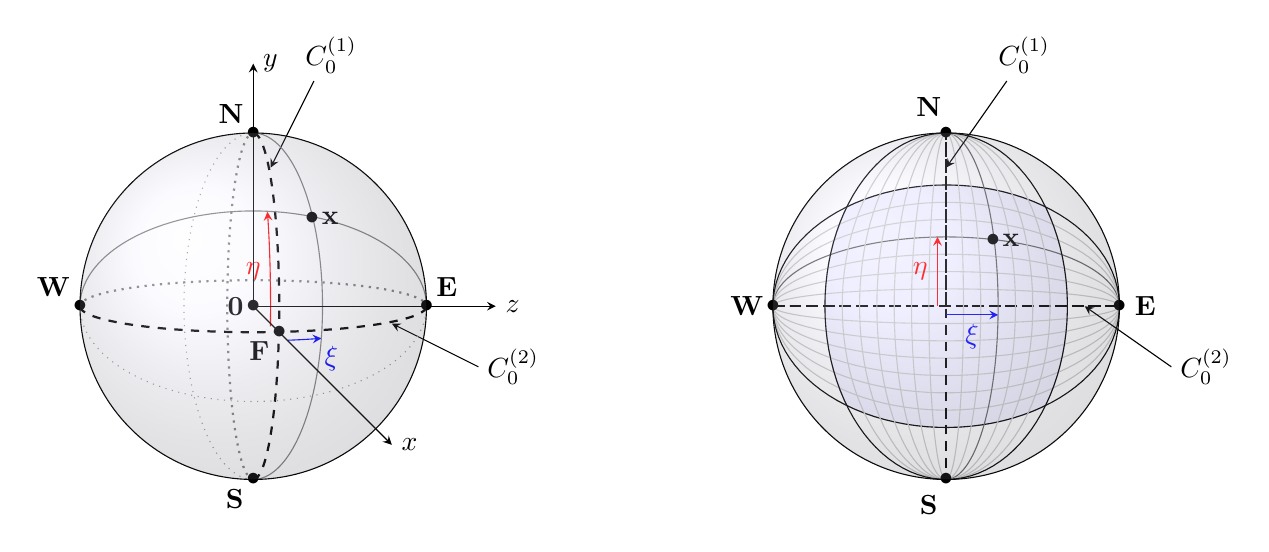
\begin{tikzpicture}[scale=2.2]
    \draw[>=stealth, ->, samples=100, color=blue, domain=-79:-68] plot({1.05*cos(\x)},{0.2*sin(\x)});
    \draw[color=blue] (.45,-.3) node{$\xi$} ;
    \draw[>=stealth, ->, samples=100, color=red, domain=-7:35] plot({0.1*cos(\x)},{0.95*sin(\x)});
    \draw[color=red] (0,0.2) node{$\eta$} ;

	\draw [dashed, line width=0.8pt, samples=100, domain=-180:0] plot({cos(\x)},{0.15*sin(\x)});
	\draw [dotted, line width=0.8pt, samples=100, domain=-180:0, color=gray] plot({cos(\x)},{-0.15*sin(\x)});
	\draw [dashed, line width=0.8pt, samples=100,domain=-90:90] plot({0.15*cos(\x)},{sin(\x)});
	\draw [dotted, line width=0.8pt, samples=100,domain=-90:90, color=gray] plot({-0.15*cos(\x)},{sin(\x)});
	\draw [>=stealth, ->] (1.3,-.35) -- (0.8,-0.1) ;
	\draw  (1.5,-.35) node {$C_0^{(2)}$} ;
	\draw [>=stealth, ->] (0.35,1.3) -- (0.1,0.8) ;
	\draw  (.45,1.45) node {$C_0^{(1)}$} ;
    
    
	\draw [samples=100, domain=-180:0, color=gray] plot({cos(\x)},{-0.55*sin(\x)});
	\draw [dotted, samples=100, domain=-180:0, color=gray!80] plot({cos(\x)},{0.55*sin(\x)});
	\draw [samples=100, domain=-90:90, color=gray] plot({0.4*cos(\x)},{sin(\x)});
	\draw [dotted, samples=100, domain=-90:90, color=gray!80] plot({-0.4*cos(\x)},{sin(\x)});
	\draw (.34,0.51) node {$\bullet$} ;
	\draw (.34,0.51) node[right]{$\mathbf{x}$} ;
	
	\draw (1,0) node {$\bullet$} ;
	\draw (1,0) node[above right]{$\mathbf{E}$} ;
	\draw (-1,0) node {$\bullet$} ;
	\draw (-1,0) node[above left]{$\mathbf{W}$} ;
	\draw (0,1) node {$\bullet$} ;
	\draw (0,1) node[above left]{$\mathbf{N}$} ;
	\draw (0,-1) node {$\bullet$} ;
	\draw (0,-1) node[below left]{$\mathbf{S}$} ;
	\draw (.15,-0.15) node {$\bullet$} ;
	\draw (.15,-0.15) node[below left]{$\mathbf{F}$} ;
	\draw (0,0) node {$\bullet$} ;
	\draw (0,0) node[left]{$\mathbf{0}$} ;
	
	\draw [>=stealth, ->] (0,0) -- (0,1.4) ;
	\draw  (0,1.4) node[right] {$y$} ;
	\draw [>=stealth, ->] (0,0) -- (1.4,0) ;
	\draw  (1.4,0) node[right] {$z$} ;
	\draw [>=stealth, ->] (0,0) -- (.8,-0.8) ;
	\draw  (.8,-0.8) node[right] {$x$} ;
	
	
    \draw (0,0) circle (1cm);
    \shade[ball color=blue!10!white,opacity=0.20] (0,0) circle (1cm);
    
    
    
    
    
    
    \filldraw[draw=black,fill=blue!30!white,opacity=0.20]
	plot [smooth,domain=-35:35] ({4+0.7*cos(\x)},{sin(\x)})
	-- plot [smooth,domain=55:125] ({4+cos(\x)},{0.7*sin(\x)})
	-- plot [smooth,domain=140:215] ({4+0.7*cos(\x)},{sin(\x)})
	-- plot [smooth,domain=230:305] ({4+cos(\x)},{0.7*sin(\x)})
	-- cycle;	
	
	\draw [dashed, line width=0.8pt, samples=100,domain=180:-180] plot({4+cos(\x)},{0*sin(\x)});
	\draw [samples=100,domain=180:-180,color=gray!40] plot({4+cos(\x)},{0.1*sin(\x)});
	\draw [samples=100,domain=180:-180,color=gray!40] plot({4+cos(\x)},{0.2*sin(\x)});
	\draw [samples=100,domain=180:-180,color=gray!40] plot({4+cos(\x)},{0.3*sin(\x)});
	\draw [samples=100,domain=180:0,color=gray!120] plot({4+cos(\x)},{0.4*sin(\x)});
	\draw [samples=100,domain=0:-180,color=gray!40] plot({4+cos(\x)},{0.4*sin(\x)});
	\draw [samples=100,domain=180:-180,color=gray!40] plot({4+cos(\x)},{0.5*sin(\x)});
	\draw [samples=100,domain=180:-180,color=gray!40] plot({4+cos(\x)},{0.6*sin(\x)});
	\draw [samples=100,domain=180:-180] plot({4+cos(\x)},{0.7*sin(\x)});
	\draw [dashed, line width=0.8pt, samples=100,domain=180:-180] plot({4+0*cos(\x)},{sin(\x)});
	\draw [samples=100,domain=180:-180,color=gray!40] plot({4+0.1*cos(\x)},{sin(\x)});
	\draw [samples=100,domain=180:-180,color=gray!40] plot({4+0.2*cos(\x)},{sin(\x)});
	\draw [samples=100,domain=-90:90,color=gray!120] plot({4+0.3*cos(\x)},{sin(\x)});
	\draw [samples=100,domain=90:270,color=gray!40] plot({4+0.3*cos(\x)},{sin(\x)});
	\draw [samples=100,domain=180:-180,color=gray!40] plot({4+0.4*cos(\x)},{sin(\x)});
	\draw [samples=100,domain=180:-180,color=gray!40] plot({4+0.5*cos(\x)},{sin(\x)});
	\draw [samples=100,domain=180:-180,color=gray!40] plot({4+0.6*cos(\x)},{sin(\x)});
	\draw [samples=100,domain=180:-180] plot({4+0.7*cos(\x)},{sin(\x)}); 
	
	\draw [>=stealth, ->] (5.3,-.35) -- (4.8,-0) ;
	\draw  (5.5,-.35) node {$C_0^{(2)}$} ;
	\draw [>=stealth, ->] (4.35,1.3) -- (4,0.8) ;
	\draw  (4.45,1.45) node {$C_0^{(1)}$} ;
	\draw  (4,1) node {$\bullet$} ;
	\draw  (3.9,1.15) node {$\mathbf{N}$} ;
	\draw  (4,-1) node {$\bullet$} ;
	\draw  (3.9,-1.15) node {$\mathbf{S}$} ;
	\draw  (5,0) node {$\bullet$} ;
	\draw  (5.15,0) node {$\mathbf{E}$} ;
	\draw  (3,0) node {$\bullet$} ;
	\draw  (4-1.15,0) node {$\mathbf{W}$} ;
	
	\draw  (4.27,0.38) node {$\bullet$} ;
	\draw  (4.27,0.38) node[right] {$\mathbf{x}$} ;
	\draw [>=stealth, ->, color=blue] (4,-0.05) -- (4.3,-0.05) ;
	\draw  (4.15,-0.05) node[color=blue, below] {$\xi$} ;
	\draw [>=stealth, ->, color=red] (3.95,0) -- (3.95,0.4) ;
	\draw  (3.95,0.2) node[color=red, left] {$\eta$} ;

	\draw (4,0) circle (1cm);
    \shade[ball color=blue!10!white,opacity=0.20] (4,0) circle (1cm);  
   
\end{tikzpicture}
\end{center}
\caption{Sur un panel, un point $\mathbf{x}$ est localisé par $\xi$ et $\eta$.}
\label{fig: panel I xi eta}
\end{figure}


Dans ce cadre, on note $C^{(1)}_i$ le grand cercle obtenu par rotation de $C^{(1)}_0$ d'un angle géodésique $i \Delta \xi$ autour de l'axe $(Oz)$ et $C^{(2)}_j$ le cercle obtenu par rotation de $C^{(2)}_0$ d'angle $j \Delta \eta$ autour de $(Oy)$.

Le maillage associé au panel I est constitué des points d'intersections des $N+1$ cercles $( C_i^{(1)} )_{-N/2 \leq i \leq N/2}$ et des $N+1$ cercles $(C_j^{(2)})_{-N/2 \leq j \leq N/2}$ (Voir figure \ref{fig: panel I}) sur le panel I. Le même procédé est reproduit sur chaque panel, il y a donc $(N+1)^2$ points d'intersections sur un panel.

\begin{figure}[htbp]
\begin{center}
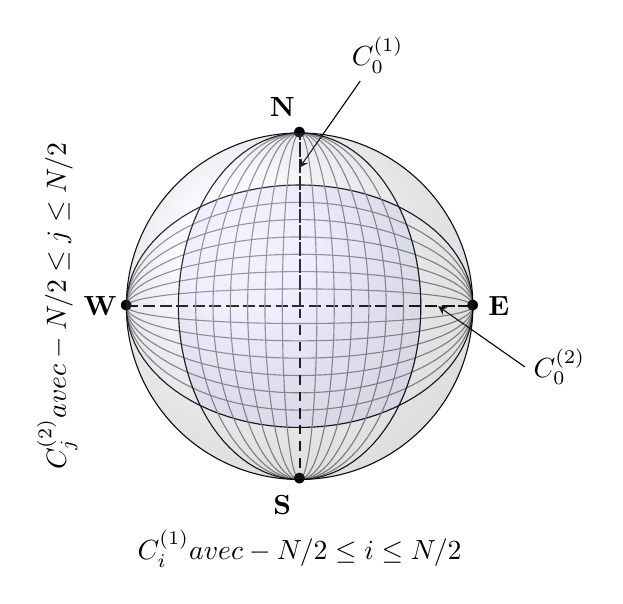
\begin{tikzpicture}[scale=2.2]
	%\draw [color=gray] (-2.5,-2.5) grid[step=0.1] (2.5,2.5);
	\filldraw[draw=black,fill=blue!30!white,opacity=0.20]
	plot [smooth,domain=-35:35] ({0.7*cos(\x)},{sin(\x)})
	-- plot [smooth,domain=55:125] ({cos(\x)},{0.7*sin(\x)})
	-- plot [smooth,domain=140:215] ({0.7*cos(\x)},{sin(\x)})
	-- plot [smooth,domain=230:305] ({cos(\x)},{0.7*sin(\x)})
	-- cycle;	
	
	\draw [dashed, line width=0.8pt, samples=100,domain=180:-180] plot({cos(\x)},{0*sin(\x)});
	\draw [samples=100,domain=180:-180,color=gray] plot({cos(\x)},{0.1*sin(\x)});
	\draw [samples=100,domain=180:-180,color=gray] plot({cos(\x)},{0.2*sin(\x)});
	\draw [samples=100,domain=180:-180,color=gray] plot({cos(\x)},{0.3*sin(\x)});
	\draw [samples=100,domain=180:-180,color=gray] plot({cos(\x)},{0.4*sin(\x)});
	\draw [samples=100,domain=180:-180,color=gray] plot({cos(\x)},{0.5*sin(\x)});
	\draw [samples=100,domain=180:-180,color=gray] plot({cos(\x)},{0.6*sin(\x)});
	\draw [samples=100,domain=180:-180] plot({cos(\x)},{0.7*sin(\x)});
	\draw [dashed, line width=0.8pt, samples=100,domain=180:-180] plot({0*cos(\x)},{sin(\x)});
	\draw [samples=100,domain=180:-180,color=gray] plot({0.1*cos(\x)},{sin(\x)});
	\draw [samples=100,domain=180:-180,color=gray] plot({0.2*cos(\x)},{sin(\x)});
	\draw [samples=100,domain=180:-180,color=gray] plot({0.3*cos(\x)},{sin(\x)});
	\draw [samples=100,domain=180:-180,color=gray] plot({0.4*cos(\x)},{sin(\x)});
	\draw [samples=100,domain=180:-180,color=gray] plot({0.5*cos(\x)},{sin(\x)});
	\draw [samples=100,domain=180:-180,color=gray] plot({0.6*cos(\x)},{sin(\x)});
	\draw [samples=100,domain=180:-180] plot({0.7*cos(\x)},{sin(\x)}); 
	
	\draw [>=stealth, ->] (1.3,-.35) -- (0.8,-0) ;
	\draw  (1.5,-.35) node {$C_0^{(2)}$} ;
	\draw [>=stealth, ->] (0.35,1.3) -- (0,0.8) ;
	\draw  (0.45,1.45) node {$C_0^{(1)}$} ;
	\draw  (0,1) node {$\bullet$} ;
	\draw  (-0.1,1.15) node {$\mathbf{N}$} ;
	\draw  (0,-1) node {$\bullet$} ;
	\draw  (-0.1,-1.15) node {$\mathbf{S}$} ;
	\draw  (1,0) node {$\bullet$} ;
	\draw  (1.15,0) node {$\mathbf{E}$} ;
	\draw  (-1,0) node {$\bullet$} ;
	\draw  (-1.15,0) node {$\mathbf{W}$} ;

	\draw (0,0) circle (1cm);
    \shade[ball color=blue!10!white,opacity=0.20] (0,0) circle (1cm);
    
    \draw  (-1.4,0) node[rotate=90] {$ C_j^{(2)}\text{ avec }-N/2\leq j \leq N/2$} ;
    \draw  (0,-1.4) node {$ C_i^{(1)}\text{ avec }-N/2\leq i \leq N/2$} ;

\end{tikzpicture}
\end{center}
\caption{Le panel I est constitué des points d'intersections d'un ensemble de grands cercles.}
\label{fig: panel I}
\end{figure}  

En reproduisant le procédé pour chaque panel, on constitue la Cubed-Sphere associée à la base $(\mathbf{i},\mathbf{j},\mathbf{k})$ et de paramètre $N$.

\begin{definition}
La Cubed-Sphere est une grille de la sphère $\mathbb{S}_a^2$. La sphère est couverte par 6 panels identiques notés panel I (Front), II (East), III (Bottom), IV (West), V (North) et VI (South). Chaque panel est doté d'un système de coordonnées :
\begin{equation}
\left( \xi^{(k)}, \eta^{(k)} \right) \text{, } -\dfrac{\pi}{4} \leq \xi^{(k)}, \eta^{(k)} \leq \dfrac{\pi}{4} \text{, } I \leq k \leq VI
\end{equation}
définis précédemment. Les points de la Cubed-Sphere sont notés $\mathbf{x}_{i,j}^{(k)}$. Ils sont définis par leurs coordonnées $\left( \xi_i^{(k)}, \eta_j^{(k)}  \right)$ avec :
\begin{equation}
\xi_i^{(k)} = i \Delta \xi \text{, } \eta_j^{(k)} = j \Delta \eta \text{, } -N/2 \leq i, j \leq N/2 \text{ et } I \leq k \leq VI,
\end{equation}
où le pas de discrétisation est :
\begin{equation}
\Delta \xi = \Delta \eta = \dfrac{\pi}{2 N}.
\end{equation}
\end{definition}

\begin{proposition}
La Cubed-Sphere est composée de $6N^2 +2$ points.
\end{proposition}

\begin{proof}
Il y a 6 intérieurs de panels de $(N-1)^2$ points, 12 arrêtes de $N-1$ points et 8 sommets. Ainsi le nombre de points sur la Cubed-Sphere est :
$$
6 (N-1)^2 + 12 (N-1)+8=6N^2+2
$$
\end{proof}

Les points $\mathbf{x}_{i,j}^{(k)}$ de chaque panel se divisent en 3 catégories :
\begin{itemize}
\item Les points intérieurs si :
\begin{equation}
- \dfrac{N}{2}+1 \leq i,j \leq \dfrac{N}{2}-1
\end{equation}
Ils sont au nombre de $(N-1)^2$ par panel.
\item Les $4(N-1)$ points de bords de chaque panel, si :
\begin{equation}
\left[ j=\pm \dfrac{N}{2} \text{ et } - \dfrac{N}{2}+1 \leq i \leq \dfrac{N}{2}-1 \right] \text{ ou } \left[ i=\pm \dfrac{N}{2} \text{ et } - \dfrac{N}{2}+1 \leq j \leq \dfrac{N}{2}-1 \right]
\end{equation}
\item Les $4$ points de coins si :
\begin{equation}
i, j = \pm \dfrac{N}{2}.
\end{equation}
\end{itemize}



\begin{figure}
\begin{center}
\includegraphics[scale=0.6]{plot_CS}
\end{center}
\caption{Cubed-Sphere avec $N=16$.}
\end{figure}















\section{Coordonnées Gnomoniques}

On considère un cube inscrit dans la Sphère $\mathbb{S}_a^2$. Le demi côté de ce cube mesure $R=\frac{\sqrt{3}}{3}a$. Chaque face du cube est donnée par :
\begin{itemize}
\item la face centrée sur $F'=(R,0,0)$ : 
\begin{equation}
\left\lbrace
\mathbf{x}' = (R,y',z') \in \mathbb{R}^3 \text{ tels que } -R  \leq y',z' \leq R
\right\rbrace
\end{equation}

\item la face centrée sur $B'=(-R,0,0)$ : 
\begin{equation}
\left\lbrace
\mathbf{x}' = (-R,y',z') \in \mathbb{R}^3 \text{ tels que } -R  \leq y',z' \leq R
\right\rbrace
\end{equation}

\item la face centrée sur $E'=(0,R,0)$ : 
\begin{equation}
\left\lbrace
\mathbf{x}' = (x',R,z') \in \mathbb{R}^3 \text{ tels que } -R  \leq x',z' \leq R
\right\rbrace
\end{equation}

\item la face centrée sur $W'=(0,-R,0)$ : 
\begin{equation}
\left\lbrace
\mathbf{x}' = (x',-R,z') \in \mathbb{R}^3 \text{ tels que } -R  \leq x',z' \leq R
\right\rbrace
\end{equation}

\item la face centrée sur $N'=(0,0,R)$ : 
\begin{equation}
\left\lbrace
\mathbf{x}' = (x',y',R) \in \mathbb{R}^3 \text{ tels que } -R  \leq x',y' \leq R
\right\rbrace
\end{equation}

\item la face centrée sur $S'=(0,0,-R)$ : 
\begin{equation}
\left\lbrace
\mathbf{x}' = (x',y',-R) \in \mathbb{R}^3 \text{ tels que } -R  \leq x',y' \leq R
\right\rbrace
\end{equation}
\end{itemize}

$\mathbf{F}$ est la projection gnomonique de $F'$ sur la sphère $\mathbb{S}_a^2$, $\mathbf{E}$ celle de $E'$, ...
Si l'on considère par exemple le panel I, un point $\mathbf{x}'=(x',y',z')$ de la face centré sur $F'$ est projeté en $\mathbf{x} = (x,y,z)$ un point du panel I (Voir figure \ref{fig: projection gnomonique}). Chaque panel est la projection de l'une des face du cube.

\begin{figure}[htbp]
\begin{center}
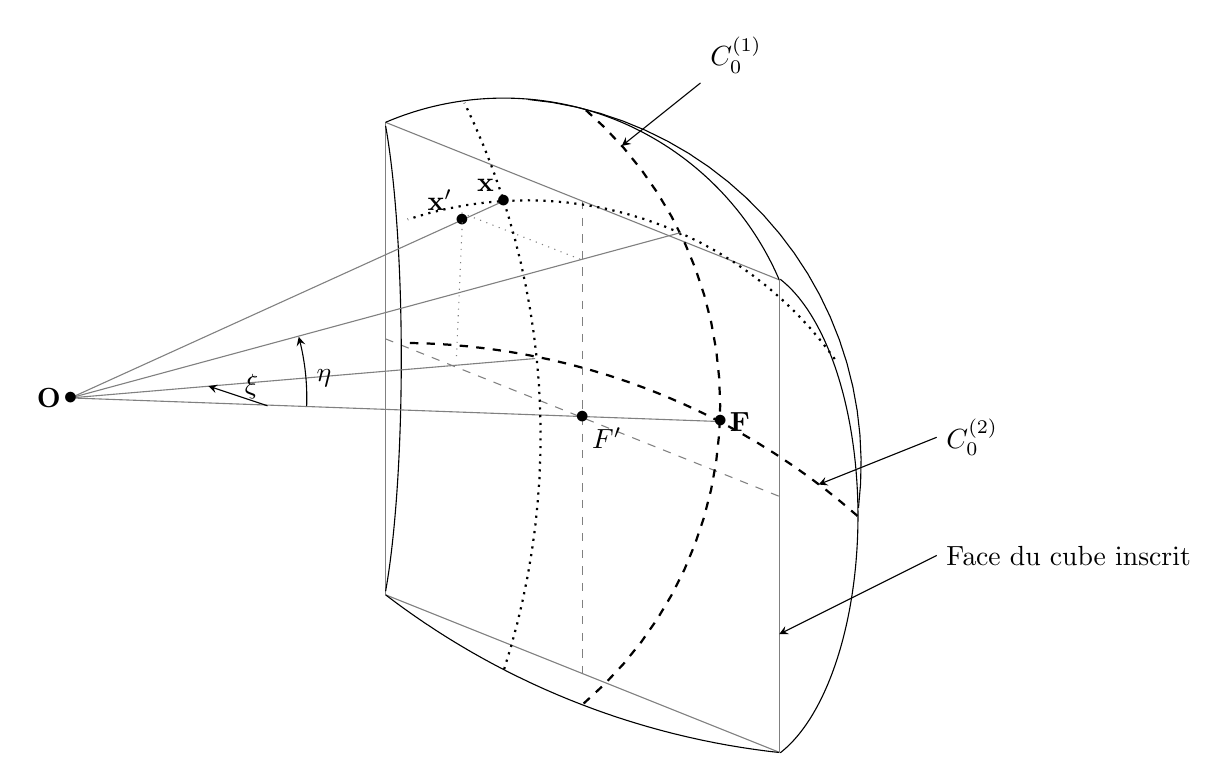
\begin{tikzpicture}[scale=1]
	\draw [color=gray] (0,3) -- (0,-3) ;
	\draw [color=gray] (0,-3) -- (5,-5) ;
	\draw [color=gray] (5,-5) -- (5,1) ;
	\draw [color=gray] (5,1) -- (0,3) ;
	\draw [dashed, color=gray] (0,.25) -- (5,-1.75) ;
	\draw [dashed, color=gray] (2.5,2) -- (2.5,-4) ;
	
	\draw [samples=100,domain=-70:70] plot({4.5+1.5*cos(\x)},{-2+3.2*sin(\x)});
	\draw [samples=100,domain=-53:53] plot({-0.3+0.5*cos(\x)},{3.7*sin(\x)});
	\draw [samples=100,domain=113.2:23.2] plot({1.5+sqrt(14.5)*cos(\x)},{-.5+sqrt(14.5)*sin(\x)});
	\draw [samples=100,domain=-96.24:-127.41] plot({6.09+sqrt(100.46)*cos(\x)},{4.96+sqrt(100.46)*sin(\x)});
	
	\draw [shift={(1.39,-1.34)}] plot[domain=-0.12:1.48,variable=\t]({1*4.65*cos(\t r)+0*4.65*sin(\t r)},{0*4.65*cos(\t r)+1*4.65*sin(\t r)});
	
	
	\draw [color=gray] (-4,-.5) -- (4.25,-0.8) ;
	\draw  (2.5,-.75) node {$\bullet$} ;
	\draw  (2.5,-.75) node[below right] {$F'$} ;
	\draw  (4.25,-0.8) node {$\bullet$} ;
	\draw  (4.25,-0.8) node[right] {$\mathbf{F}$} ;
	
	\draw [dashed, line width=0.8pt, shift={(-0.74,-0.6)}] plot[domain=-0.86:0.86,variable=\t]({1*4.99*cos(\t r)+0*4.99*sin(\t r)},{0*4.99*cos(\t r)+1*4.99*sin(\t r)});
	\draw [dashed, line width=0.8pt, shift={(0.16,-8.64)}] plot[domain=0.85:1.56,variable=\t]({1*8.84*cos(\t r)+0*8.84*sin(\t r)},{0*8.84*cos(\t r)+1*8.84*sin(\t r)});
	
	\draw [color=gray] (-4,-.5) -- (1.5,2) ;
	\draw  (1.5,2) node {$\bullet$} ;
	\draw  (1.5,2) node[above left] {$\textbf{x}$} ;
	
	\draw [dotted, line width=0.8pt, shift={(1.79,-2.8)}] plot[domain=0.62:1.89,variable=\t]({1*4.81*cos(\t r)+0*4.81*sin(\t r)},{0*4.81*cos(\t r)+1*4.81*sin(\t r)});
	\draw [dotted, line width=0.8pt, shift={(-7.75,-0.98)}] plot[domain=-0.31:0.45,variable=\t]({1*9.72*cos(\t r)+0*9.72*sin(\t r)},{0*9.72*cos(\t r)+1*9.72*sin(\t r)});

	\draw [color=gray] (-4,-.5) -- (1.9,0) ;
	\draw [color=gray] (-4,-.5) -- (3.75,1.6) ;
	
	\draw  (.97,1.75) node {$\bullet$} ;
	\draw  (.97,1.75) node[above left] {$\textbf{x}'$} ;
	\draw [dotted, color=gray] (.965,1.85) -- (2.5,1.25) ;
	\draw [dotted, color=gray] (.975,1.73) -- (.9,0) ;
	
	\draw  (-4,-.5) node {$\bullet$} ;
	\draw  (-4,-.5) node[left] {$\mathbf{O}$} ;
	
	\draw [>=stealth, ->] (-1.5,-.6) -- (-2.25,-.35) ;
	\draw  (-1.7,-.35) node {$\xi$} ;
	\draw [>=stealth, ->,domain=-2:15] plot({-4+3*cos(\x)},{-.5+3*sin(\x)});
	\draw  (-1,-.25) node[right] {$\eta$} ;
	
	\draw [>=stealth, <-] (5.5,-1.6) -- (7,-1) ;
	\draw  (7,-1) node[right] {$C_0^{(2)}$} ;
	\draw [>=stealth, <-] (3,2.7) -- (4,3.5) ;
	\draw  (4,3.5) node[above right] {$C_0^{(1)}$} ;
	\draw [>=stealth, <-] (5,-3.5) -- (7,-2.5) ;
	\draw  (7,-2.5) node[right] {Face du cube inscrit} ;

\end{tikzpicture}
\end{center}
\caption{Projection gnomonique.}
\label{fig: projection gnomonique}
\end{figure}  

On constate alors les relations suivantes :
\begin{equation}
\tan \xi = \dfrac{y'}{x'} = \dfrac{y}{x} \text{ et } \tan \eta = \dfrac{z'}{x'} = \dfrac{z}{x}
\end{equation}

Or $\mathbf{x}'(x',y',z')$ est un point de la face du cube centrée en $F'$, donc $x'=R=\frac{\sqrt{3}}{6}a$ :
\begin{equation}
\tan \xi = \dfrac{y'}{R} = \dfrac{y}{x} \text{ et } \tan \eta = \dfrac{z'}{R} = \dfrac{z}{x}
\end{equation}

Quel que soit la face, on définit $(X,Y)$ les coordonnées gnomoniques.

\begin{definition}
Les coordonnées gnomoniques $(X,Y) \in [-1,1]^2$ sont définies par :
\begin{equation}
X:=\tan \xi \text{ et } Y:= \tan \eta.
\end{equation}
\end{definition}

Un point de la sphère est localisé de manière unique par sa face et ses coordonnées gnomoniques. Si on se donne $(X,Y)$ un couple de coordonnées gnomoniques du panel I, on a :

\begin{equation}
\left\lbrace
\begin{array}{rcl}
x^2+y^2+z^2 & = & a^2\\
X & = & \dfrac{y}{x} \\
Y & = & \dfrac{z}{x}
\end{array}
\right.
\end{equation}

ainsi $x^2 \left( 1+X^2+Y^2 \right) = a^2$, d'où :

\begin{equation}
\left\lbrace
\begin{array}{rclcl}
x & = & \pm \dfrac{a}{\sqrt{1+X^2+Y^2}}& = & \dfrac{a}{\sqrt{1+X^2+Y^2}}\\
y & = & xX &&\\
z & = & xY &&
\end{array}
\right.
\end{equation}

le signe de $x$ est donné car $\mathbf{x}$ est un point du panel I qui ne contient que des points d'abscisse positive.
De plus, $\tan$ est une bijection de $\left[ -\dfrac{\pi}{4}, \dfrac{\pi}{4} \right]$ dans $\left[-1,1\right]$, donc

\begin{theoreme}
Pour chaque panel, les coordonnées gnomoniques $(X,Y) \in [-1,1]^2$ et $(\xi, \eta) \in \left[ - \dfrac{\pi}{4}, \dfrac{\pi}{4} \right]^2$ forment des systèmes de coordonnées admissibles.
\end{theoreme}

De là, on peut dériver les coordonnées de $\mathbb{R}^3$ d'un point $\mathbf{x}(x,y,z)$ en fonction de $\xi$ et $\eta$ :

\begin{equation}
\dfrac{\partial y}{\partial \xi} = \dfrac{\partial x}{\partial \xi} X + x \dfrac{\partial X}{\partial \xi} = \dfrac{\partial x}{\partial \xi} X + x(1+X^2)
\end{equation}

\begin{equation}
\dfrac{\partial z}{\partial \xi} = \dfrac{\partial x}{\partial \xi} Y + x \dfrac{\partial Y}{\partial \xi} = \dfrac{\partial x}{\partial \xi} Y
\end{equation}

Le calcul de ces dérivées dépend de $\dfrac{\partial x}{\partial \xi}$ :

\begin{equation*}
\begin{array}{rcl}
0 & = & \dfrac{\partial}{\partial \xi} ( x^2+y^2+z^2) \\
  & = & 2x\dfrac{\partial x}{\partial \xi} + 2y\dfrac{\partial y}{\partial \xi}+ 2z\dfrac{\partial z}{\partial \xi} \\
  & = & x \dfrac{\partial x}{\partial \xi} ( 1 +X^2 + Y^2) + x^2 X (1+X^2)\\
  & = & x \dfrac{\partial x}{\partial \xi} \delta^2 + xy (1+X^2)
\end{array}
\end{equation*}

en posant $\delta = \sqrt{1+X^2+Y^2}$. Ainsi, chaque dérivée est connue et :

\begin{equation}
\left\lbrace
\begin{array}{rcl}
\dfrac{\partial x}{\partial \xi} & = & -\dfrac{y(1+X^2)}{\delta^2}\\
\dfrac{\partial y}{\partial \xi} & = & x \dfrac{1+X^2}{\delta^2} (1+Y^2)\\
\dfrac{\partial z}{\partial \xi} & = & - \dfrac{yY(1+X^2)}{\delta^2}
\end{array}
\right.
\end{equation}

De la même manière, en dérivant par rapport à $\eta$ :

\begin{equation}
\left\lbrace
\begin{array}{rcl}
\dfrac{\partial x}{\partial \eta} & = & - z\dfrac{1+Y^2}{\delta^2}\\
\dfrac{\partial y}{\partial \eta} & = & - zX\dfrac{1+Y^2}{\delta^2}\\
\dfrac{\partial z}{\partial \eta} & = & - x(1+X^2) \dfrac{1+Y^2}{\delta^2}
\end{array}
\right.
\end{equation}

On en déduit la base sur le panel I $\left( \mathbf{g}_{\xi}, \mathbf{g}_{\eta} \right)$ donnée par :

\begin{equation}
\mathbf{g}_{\xi} := \dfrac{\partial \mathbf{x}}{\partial \xi}= \dfrac{1+X^2}{\delta^2} \begin{bmatrix}
-y \\ x(1+Y^2) \\ -yY
\end{bmatrix} \text{ et } \mathbf{g}_{\eta} := \dfrac{\partial \mathbf{x}}{\partial \xi}= \dfrac{1+Y^2}{\delta^2} \begin{bmatrix}
-z \\ -zX \\ x(1+X^2)
\end{bmatrix}
\label{eq: base locale I}
\end{equation}

Des calculs similaires peuvent être effectuées sur les autres panels. Les résultats sont donnés dans le tableau \ref{tab: base g_xi g_eta}.

$(\mathbf{g}^{\xi}, \mathbf{g}^{\eta})$ est la base duale de $(\mathbf{g}_{\xi}, \mathbf{g}_{\eta})$. Cette base doit vérifier les relations suivantes :

\begin{equation}
\left\lbrace
\begin{array}{rcccl}
\mathbf{g}^{\xi} \cdot \mathbf{g}_{\xi} & = & 1 & = & \mathbf{g}^{\eta} \cdot \mathbf{g}_{\eta} \\
\mathbf{g}^{\xi} \cdot \mathbf{g}_{\eta} & = & 0 & = & \mathbf{g}^{\eta} \cdot \mathbf{g}_{\xi} \\
\end{array}
\right.
\label{eq: normalisation g_xi g_eta}
\end{equation}

$\mathbf{g}^{\xi}$ et $\mathbf{g}^{\eta}$ sont des vecteurs de $\mathbb{T}_{\mathbf{x}}\mathbb{S}_a^2$. Il existe $A$, $B$, $C$ et $D$ tels que :

\begin{equation}
\left\lbrace
\begin{array}{rcl}
\mathbf{g}^{\xi} & = & A \mathbf{g}_{\xi} + B \mathbf{g}_{\eta} \\
\mathbf{g}^{\eta} & = & C \mathbf{g}_{\xi} + D \mathbf{g}_{\eta} \\
\end{array}
\right.
\label{eq: A B C D}
\end{equation}

En effectuant des produit scalaires de \eqref{eq: A B C D} par $\mathbf{g}_{\xi}$ et $\mathbf{g}_{\eta}$, on montre que :

\begin{equation}
\begin{bmatrix}
A & B \\ C &  D
\end{bmatrix}
\times
\begin{bmatrix}
\mathbf{g}_{\xi} \cdot \mathbf{g}_{\xi} & \mathbf{g}_{\xi} \cdot \mathbf{g}_{\eta} \\
\mathbf{g}_{\eta} \cdot \mathbf{g}_{\xi} & \mathbf{g}_{\eta} \cdot \mathbf{g}_{\eta}
\end{bmatrix}
= \begin{bmatrix}
1 & 0 \\ 0 &  1
\end{bmatrix}
\end{equation}

On peut directement déduire :
\begin{equation}
\begin{bmatrix}
A & B \\ C &  D
\end{bmatrix} 
=
\begin{bmatrix}
\mathbf{g}_{\xi} \cdot \mathbf{g}_{\xi} & \mathbf{g}_{\xi} \cdot \mathbf{g}_{\eta} \\
\mathbf{g}_{\eta} \cdot \mathbf{g}_{\xi} & \mathbf{g}_{\eta} \cdot \mathbf{g}_{\eta}
\end{bmatrix}^{-1}
\end{equation}


\begin{definition}
$\mathbf{G}$ est la métrique associée à $(\mathbf{g}_{\xi}, \mathbf{g}_{\eta})$ en $\mathbf{x}$:
\begin{equation}
\mathbf{G} = \begin{bmatrix}
\mathbf{g}_{\xi} \cdot \mathbf{g}_{\xi} & \mathbf{g}_{\xi} \cdot \mathbf{g}_{\eta} \\
\mathbf{g}_{\eta} \cdot \mathbf{g}_{\xi} & \mathbf{g}_{\eta} \cdot \mathbf{g}_{\eta}
\end{bmatrix}
\end{equation}
\end{definition}

\begin{proposition}
La métrique $\mathbf{G}$ est invariante par changement de panel.
\end{proposition}

\begin{proof}
Soit $\mathbf{x}$ est un point d'un panel $K$ de la Cubed-Sphère de coordonnées gnomoniques $(X,Y)$ et $\mathbf{x}'$ est un point d'un autre panel $K'$ de la Cubed-Sphère ayant les mêmes coordonnées gnomoniques $(X,Y)$. Il existe une rotation $R_f$ qui permet de transformer tout point du panel $K$ en un point du panel $K'$ de mêmes coordonnées gnomoniques. De là, il découle :
\begin{equation}
\mathbf{x}' = R_f \mathbf{x}
\end{equation}
Cette rotation est indépendante de $\xi$ et de $\eta$. Donc :
\begin{equation}
\mathbf{g'}_{\xi} = \dfrac{\partial}{\partial \xi} \left( R_f \mathbf{x} \right) = R_f \dfrac{\partial \mathbf{x}}{\partial \xi}  = R_f \mathbf{g}_{\xi}
\end{equation}
De même, on a $\mathbf{g'}_{\eta} = R_f\mathbf{g}_{\eta}$.
Ainsi, si $\mathbf{G}$ est la métrique en $\mathbf{x}$ et $\mathbf{G}'$ la métrique en $\mathbf{x}'$, on a :

\begin{equation*}
\begin{array}{rcl}
\mathbf{G}' &=& \begin{bmatrix}
\mathbf{g'}_{\xi} \cdot \mathbf{g'}_{\xi} & \mathbf{g'}_{\xi} \cdot \mathbf{g'}_{\eta} \\
\mathbf{g'}_{\eta} \cdot \mathbf{g'}_{\xi} & \mathbf{g'}_{\eta} \cdot \mathbf{g'}_{\eta}
\end{bmatrix}\\[10pt]
&=&
\begin{bmatrix}
R_f \mathbf{g}_{\xi} \cdot R_f \mathbf{g}_{\xi} & R_f \mathbf{g}_{\xi} \cdot R_f \mathbf{g}_{\eta} \\
R_f \mathbf{g}_{\eta} \cdot R_f \mathbf{g}_{\xi} & R_f \mathbf{g}_{\eta} \cdot R_f \mathbf{g}_{\eta}
\end{bmatrix}\\[10pt]
&=&
\begin{bmatrix}
\mathbf{g}_{\xi} \cdot R_f^{T} R_f \mathbf{g}_{\xi} & \mathbf{g}_{\xi} \cdot  R_f^{T} R_f \mathbf{g}_{\eta} \\
\mathbf{g}_{\eta} \cdot  R_f^{T} R_f \mathbf{g}_{\xi} & \mathbf{g}_{\eta} \cdot  R_f^{T} R_f \mathbf{g}_{\eta}
\end{bmatrix}\\[10pt]
&=& \begin{bmatrix}
\mathbf{g}_{\xi} \cdot \mathbf{g}_{\xi} & \mathbf{g}_{\xi} \cdot \mathbf{g}_{\eta} \\
\mathbf{g}_{\eta} \cdot \mathbf{g}_{\xi} & \mathbf{g}_{\eta} \cdot \mathbf{g}_{\eta}
\end{bmatrix}\\[10pt]
& = & \mathbf{G}
\end{array}
\end{equation*}
Donc la métrique $\mathbf{G}$ est invariante par changement de panel.
\end{proof}

Les calculs de produits scalaire se font facilement et donnent :

\begin{equation}
\mathbf{G} = \begin{bmatrix}
G_{1,1} & G_{1,2} \\ G_{2,1} & G_{2,2}
\end{bmatrix} 
= a^2 \dfrac{(1+X^2)(1+Y^2)}{\delta^4} \begin{bmatrix}
1+X^2 & -XY \\ -XY & 1+Y^2
\end{bmatrix}
\end{equation}

qui s'inverse en :

\begin{equation}
\mathbf{G}^{-1} = \begin{bmatrix}
G^{1,1} & G^{1,2} \\ G^{2,1} & G^{2,2}
\end{bmatrix} = \dfrac{\delta^2}{a^2 (1+X^2)(1+Y^2)} \begin{bmatrix}
1+Y^2 & XY \\ XY & 1+X^2
\end{bmatrix}
\label{eq: metrique inverse}
\end{equation}

La base duale $(\mathbf{g}^{\xi}, \mathbf{g}^{\eta})$ sur le panel I est donnée par :

\begin{equation}
\left\lbrace
\begin{array}{rcl}
\mathbf{g}^{\xi} & = & G^{1,1} \mathbf{g}_{\xi} + G^{1,2} \mathbf{g}_{\eta} \\
\mathbf{g}^{\eta} & = & G^{2,1} \mathbf{g}_{\eta} + G^{2,2} \mathbf{g}_{\eta}
\end{array}
\right.
\end{equation}

d'où :

\begin{equation}
\mathbf{g}^{\xi} = \dfrac{1}{x(1+X^2)}\begin{bmatrix}
-X \\ 1 \\ 0
\end{bmatrix} \text{ et } \mathbf{g}^{\eta} = \dfrac{1}{x(1+Y^2)}\begin{bmatrix}
-Y \\ 0 \\ 1
\end{bmatrix}
\label{eq: base duale I}
\end{equation}



\begin{table}[htbp]
\begin{center}
%\rotatebox{90}{
\begin{tabular}{|c|c|c|}
\hline
\textbf{Panel} & \textbf{Coord. Gnomoniques} $(X,Y)$ & \textbf{Bases } $\left( \mathbf{g}_{\xi}, \mathbf{g}_{\eta} \right)$ et $\left( \mathbf{g}^{\xi}, \mathbf{g}^{\eta} \right)$\\

\hline
\hline
\multirow{2}{*}[-.5cm]{$I$} & \multirow{2}{*}[-.5cm]{$X=\dfrac{y}{x} \text{, } Y=\dfrac{z}{x}$} & $\mathbf{g}_{\xi} = \dfrac{1+X^2}{\delta^2} \begin{bmatrix}
-y \\ x(1+Y^2) \\ -yY
\end{bmatrix} \text{,} \mathbf{g}_{\eta} = \dfrac{1+Y^2}{\delta^2} \begin{bmatrix}
-z \\ -zX \\ x(1+X^2)
\end{bmatrix}$ \\[16pt]

\cline{3-3}
& &  $\mathbf{g}^{\xi} = \dfrac{1}{x(1+X^2)}\begin{bmatrix}
-X \\ 1 \\ 0
\end{bmatrix} \text{ et } \mathbf{g}^{\eta} = \dfrac{1}{x(1+Y^2)}\begin{bmatrix}
-Y \\ 0 \\ 1
\end{bmatrix}$ \\[16pt]
\hline
\hline
\multirow{2}{*}[-.5cm]{$II$} & \multirow{2}{*}[-.5cm]{$X=-\dfrac{x}{y} \text{, } Y=\dfrac{z}{y}$} & $\mathbf{g}_{\xi} = \dfrac{1+X^2}{\delta^2} \begin{bmatrix}
-y(1+Y^2) \\ x \\ xY
\end{bmatrix} \text{, } \mathbf{g}_{\eta} = \dfrac{1+Y^2}{\delta^2} \begin{bmatrix}
zX \\ -z \\ y(1+X^2)
\end{bmatrix}$ \\[16pt]

\cline{3-3}
 & & $\mathbf{g}^{\xi} = \dfrac{1}{y(1+X^2)}\begin{bmatrix}
-1 \\ -X \\ 0
\end{bmatrix} \text{, } \mathbf{g}^{\eta} = \dfrac{1}{y(1+Y^2)}\begin{bmatrix}
0 \\ -Y \\ 1
\end{bmatrix}$ \\[16pt]
\hline
\hline
\multirow{2}{*}[-.5cm]{$III$} & \multirow{2}{*}[-.5cm]{$X=-\dfrac{y}{x} \text{, } Y=-\dfrac{z}{x}$} & $\mathbf{g}_{\xi} = \dfrac{1+X^2}{\delta^2} \begin{bmatrix}
-y \\ x(1+Y^2) \\ yY
\end{bmatrix} \text{, } \mathbf{g}_{\eta} = \dfrac{1+Y^2}{\delta^2} \begin{bmatrix}
-z \\ -zX \\ x(1+X^2)
\end{bmatrix}$ \\[16pt]

 \cline{3-3}
 &  & $\mathbf{g}^{\xi} = \dfrac{1}{x(1+X^2)}\begin{bmatrix}
-X \\ 1 \\ 0
\end{bmatrix} \text{, } \mathbf{g}^{\eta} = \dfrac{1}{x(1+Y^2)}\begin{bmatrix}
-Y \\ 0 \\ -1
\end{bmatrix}$ \\[16pt]
\hline
\hline
\multirow{2}{*}[-.5cm]{$IV$} & \multirow{2}{*}[-.5cm]{$X=\dfrac{x}{y} \text{, } Y=-\dfrac{z}{y}$} & $\mathbf{g}_{\xi} = \dfrac{1+X^2}{\delta^2} \begin{bmatrix}
-y(1+Y^2) \\ x \\ -xY
\end{bmatrix} \text{, } \mathbf{g}_{\eta} = \dfrac{1+Y^2}{\delta^2} \begin{bmatrix}
-zX \\ z \\ -y(1+X^2)
\end{bmatrix}$ \\[16pt]

\cline{3-3}
&  & $\mathbf{g}^{\xi} = \dfrac{1}{y(1+X^2)}\begin{bmatrix}
-1 \\ -X \\ 0
\end{bmatrix} \text{, } \mathbf{g}^{\eta} = \dfrac{1}{y(1+Y^2)}\begin{bmatrix}
0 \\ -Y \\ -1
\end{bmatrix}$ \\[16pt]
\hline
\hline
\multirow{2}{*}[-.5cm]{$V$} & \multirow{2}{*}[-.5cm]{$X=\dfrac{y}{z} \text{, } Y=\dfrac{x}{z}$} & $\mathbf{g}_{\xi} = \dfrac{1+X^2}{\delta^2} \begin{bmatrix}
-yY \\ z(1+Y^2) \\ -y
\end{bmatrix} \text{, } \mathbf{g}_{\eta} = \dfrac{1+Y^2}{\delta^2} \begin{bmatrix}
-z(1+X^2) \\ xX \\ x
\end{bmatrix}$ \\[16pt]

\cline{3-3}
 &  & $\mathbf{g}^{\xi} = \dfrac{1}{z(1+X^2)}\begin{bmatrix}
0 \\ 1 \\ -X
\end{bmatrix} \text{, } \mathbf{g}^{\eta} = \dfrac{1}{z(1+Y^2)}\begin{bmatrix}
-1 \\ 0 \\ -Y
\end{bmatrix}$ \\[16pt]
\hline
\hline
\multirow{2}{*}[-.5cm]{$VI$} & \multirow{2}{*}[-.5cm]{$X=-\dfrac{y}{z} \text{, } Y=-\dfrac{x}{z}$} & $\mathbf{g}_{\xi} = \dfrac{1+X^2}{\delta^2} \begin{bmatrix}
-yY \\ -z(1+Y^2) \\ y
\end{bmatrix} \text{, } \mathbf{g}_{\eta} = \dfrac{1+Y^2}{\delta^2} \begin{bmatrix}
-z(1+X^2) \\ -xX \\ x
\end{bmatrix}$ \\[16pt]

\cline{3-3}
 &  & $\mathbf{g}^{\xi} = \dfrac{1}{z(1+X^2)}\begin{bmatrix}
0 \\ -1 \\ -X
\end{bmatrix} \text{, } \mathbf{g}^{\eta} = \dfrac{1}{z(1+Y^2)}\begin{bmatrix}
-1 \\ 0 \\ -Y
\end{bmatrix}$ \\[16pt]
\hline

\end{tabular}
%}
\end{center}
\caption{Coordonnées gnomoniques en fonction de $x$, $y$ et $z$ et bases $\left( \mathbf{g}_{\xi}, \mathbf{g}_{\eta} \right)$ et $\left( \mathbf{g}^{\xi}, \mathbf{g}^{\eta} \right)$ en fonction de $x$, $y$ et $z$  sur chaque panel.}
\label{tab: base g_xi g_eta}
\end{table}

Les champs de vecteur $( \mathbf{g}^{\xi}, \mathbf{g}^{\eta})$ et $( \mathbf{g}_ {\xi}, \mathbf{g}_{\eta})$ sont tangents à la sphère et sont fonctions de $\xi$ et $\eta$. On définit les \textit{symboles de Christoffel} par :

\begin{definition}
Les symboles de Christoffel $\Gamma_{\kappa,\nu}^{\tau}$ (avec $\kappa$, $\nu$ et $\tau$ dans $\lbrace \xi, \eta \rbrace$), sont définis par :
\begin{equation}
\left\lbrace
\begin{array}{rcl}
\dfrac{\partial \mathbf{g}_{\xi}}{\partial \xi} & = & \Gamma_{\xi,\xi}^{\xi} \mathbf{g}_{\xi} + \Gamma_{\xi,\xi}^{\eta} \mathbf{g}_{\eta}+ \Gamma_{\xi, \xi}^{r} \mathbf{n}\\

\dfrac{\partial \mathbf{g}_{\xi}}{\partial \eta} & = & \Gamma_{\eta,\xi}^{\xi} \mathbf{g}_{\xi} + \Gamma_{\eta,\xi}^{\eta} \mathbf{g}_{\eta}+ \Gamma_{\eta, \xi}^{r} \mathbf{n}\\

\dfrac{\partial \mathbf{g}_{\eta}}{\partial \xi} & = & \Gamma_{\xi,\eta}^{\xi} \mathbf{g}_{\xi} + \Gamma_{\xi,\eta}^{\eta} \mathbf{g}_{\eta}+ \Gamma_{\xi, \eta}^{r} \mathbf{n}\\

\dfrac{\partial \mathbf{g}_{\eta}}{\partial \eta} & = & \Gamma_{\eta,\eta}^{\xi} \mathbf{g}_{\xi} + \Gamma_{\eta,\eta}^{\eta} \mathbf{g}_{\eta}+ \Gamma_{\eta, \eta}^{r} \mathbf{n}\\
\end{array}
\right.
\end{equation}
où $\mathbf{n}$ est le vecteur unitaire normale extérieure à la sphère $\mathbb{S}_a^2$:
\begin{equation}
\mathbf{n}= \dfrac{\mathbf{x}}{a}
\end{equation}
\end{definition}

\begin{proposition}
Les relations suivantes sont vérifiées :

\begin{equation}
\left\lbrace
\begin{array}{rcccl}
\Gamma_{\xi,\xi}^{\xi} & = & \left[ \dfrac{\partial \mathbf{g}_{\xi}}{\partial \xi} \right] \cdot \mathbf{g}^{\xi} & = & - \left[ \dfrac{\partial \mathbf{g}^{\xi}}{\partial \xi} \right] \cdot \mathbf{g}_ {\xi}\\

\Gamma_{\xi,\xi}^{\eta} & = & \left[ \dfrac{\partial \mathbf{g}_{\xi}}{\partial \xi} \right] \cdot \mathbf{g}^{\eta} & = & - \left[ \dfrac{\partial \mathbf{g}^{\eta}}{\partial \xi} \right] \cdot \mathbf{g}_ {\xi}\\

\Gamma_{\xi,\eta}^{\xi} & = & \left[ \dfrac{\partial \mathbf{g}_{\eta}}{\partial \xi} \right] \cdot \mathbf{g}^{\xi} & = & - \left[ \dfrac{\partial \mathbf{g}^{\xi}}{\partial \xi} \right] \cdot \mathbf{g}_ {\eta}\\

\Gamma_{\xi,\eta}^{\eta} & = & \left[ \dfrac{\partial \mathbf{g}_{\eta}}{\partial \xi} \right] \cdot \mathbf{g}^{\eta} & = & - \left[ \dfrac{\partial \mathbf{g}^{\eta}}{\partial \xi} \right] \cdot \mathbf{g}_ {\eta}\\

\Gamma_{\eta,\eta}^{\eta} & = & \left[ \dfrac{\partial \mathbf{g}_{\eta}}{\partial \eta} \right] \cdot \mathbf{g}^{\eta} & = & - \left[ \dfrac{\partial \mathbf{g}^{\eta}}{\partial \eta} \right] \cdot \mathbf{g}_ {\eta}\\

\Gamma_{\eta,\eta}^{\xi} & = & \left[ \dfrac{\partial \mathbf{g}_{\eta}}{\partial \eta} \right] \cdot \mathbf{g}^{\xi} & = & - \left[ \dfrac{\partial \mathbf{g}^{\xi}}{\partial \eta} \right] \cdot \mathbf{g}_ {\eta}\\

\Gamma_{\eta,\eta}^{r} & = & \left[ \dfrac{\partial \mathbf{g}_{\eta}}{\partial \eta} \right] \cdot \mathbf{n} & = & - \dfrac{1}{a}|\mathbf{g}_{\eta}|^2\\

\Gamma_{\xi,\xi}^{r} & = & \left[ \dfrac{\partial \mathbf{g}_{\xi}}{\partial \xi} \right] \cdot \mathbf{n} & = & - \dfrac{1}{a}|\mathbf{g}_{\xi}|^2\\

\Gamma_{\xi,\eta}^r & = & \left[ \dfrac{\partial \mathbf{g}_{\eta}}{\partial \xi} \right] \cdot \mathbf{n} & = & - \dfrac{1}{a} \mathbf{g}_{\eta} \cdot \mathbf{g}_{\xi} \\

\end{array}
\right.
\end{equation}
\end{proposition}

\begin{proof}
Nous ne démontrons que la première égalité, les autres se retrouvent la même manière.

$$\left[ \dfrac{\partial \mathbf{g}_{\xi}}{\partial \xi} \right] \cdot \mathbf{g}^{\xi} = \left[ \Gamma_{\xi,\xi}^{\xi} \mathbf{g}_{\xi} + \Gamma_{\xi,\xi}^{\eta} \mathbf{g}_{\eta} + \Gamma_{\xi,\xi}^r \mathbf{n}\right] \cdot \mathbf{g}^{\xi}$$

Or $\mathbf{g}_{\xi} \cdot \mathbf{g}^{\xi} = 1$ et $\mathbf{g}_{\eta} \cdot \mathbf{g}^{\xi} = 0$, d'où la première partie :

$$\Gamma_{\xi,\xi}^{\xi} = \left[ \dfrac{\partial \mathbf{g}_{\xi}}{\partial \xi} \right] \cdot \mathbf{g}^{\xi}.$$

D'autres part, on a :

$$\Gamma_{\xi,\xi}^{\xi} = \left[ \dfrac{\partial \mathbf{g}_{\xi}}{\partial \xi} \right] \cdot \mathbf{g}^{\xi} = \dfrac{\partial}{\partial \xi}  \underbrace{\left(\mathbf{g}_{\xi} \cdot \mathbf{g}^{\xi}\right)}_{=1}  - \left[ \dfrac{\partial \mathbf{g}^{\xi}}{\partial \xi}  \right] \cdot \mathbf{g}_{\xi} = - \left[ \dfrac{\partial \mathbf{g}^{\xi}}{\partial \xi}  \right] \cdot \mathbf{g}_{\xi}$$

et la relation est démontrée.
\end{proof}

\begin{remarque}
On note que $\Gamma_{\eta,\xi}^{\xi}=\Gamma_{\xi,\eta}^{\xi}$ et $\Gamma_{\eta,\xi}^{\eta}=\Gamma_{\xi,\eta}^{\eta}$.

En effet :
$$\Gamma_{\xi, \eta}^{\eta} = \left( \dfrac{\partial \mathbf{g}_{\eta}}{\partial \xi} \right) \cdot \mathbf{g}^{\eta} = \left( \dfrac{\partial}{\partial \xi} \dfrac{\partial \mathbf{x}}{\partial \eta} \right) \cdot \mathbf{g}^{\eta} = \left( \dfrac{\partial}{\partial \eta} \dfrac{\partial \mathbf{x}}{\partial \xi} \right) \cdot \mathbf{g}^{\eta} = \left( \dfrac{\partial \mathbf{g}_{\xi}}{\partial \eta} \right) \cdot \mathbf{g}^{\eta} = \Gamma_{\eta, \xi}^{\eta}$$

de même pour $\Gamma_{\eta,\xi}^{\xi}=\Gamma_{\xi,\eta}^{\xi}$ et $\Gamma_{\eta,\xi}^{r}=\Gamma_{\xi,\eta}^{r}$.
\end{remarque}


On peut calculer les dérivées suivantes :

\begin{equation}
\dfrac{\partial \mathbf{g}^{\xi}}{\partial \xi} = \dfrac{1}{\delta^2 x (1+X^2)} \begin{bmatrix}
X^2Y^2 - \delta^2 \\ -X(Y^2+\delta^2) \\ 0
\end{bmatrix}
\text{ et }
\dfrac{\partial \mathbf{g}^{\xi}}{\partial \eta} = \dfrac{1+Y^2}{\delta^2 x^2 (1+X^2)} \begin{bmatrix}
-X \\ 1 \\ 0
\end{bmatrix}
\end{equation}

de même :

\begin{equation}
\dfrac{\partial \mathbf{g}^{\eta}}{\partial \xi} = \dfrac{X(1+X^2)}{x \delta^2 (1+Y^2)} \begin{bmatrix}
-Y \\ 0 \\ 1
\end{bmatrix}
\text{ et }
\dfrac{\partial \mathbf{g}^{\eta}}{\partial \eta} = \dfrac{1}{x \delta^2 (1+Y^2)} \begin{bmatrix}
X^2 Y^2 - \delta^2 \\ 0 \\ -Y(X^2 - \delta^2)
\end{bmatrix}
\end{equation}

d'où les symboles de Christoffel :

\begin{equation}
\left\lbrace
\begin{array}{rcl}
\Gamma_{\xi,\eta}^{\xi} & = & - \dfrac{Y ( 1+Y^2)}{\delta^2}\\
\Gamma_{\xi,\eta}^{\eta} & = & - \dfrac{X(1+X^2)}{\delta^2}\\
\Gamma_{\eta,\eta}^{\xi} & = & 0 \\
\Gamma_{\xi,\xi}^{\eta} & = & 0 \\
\Gamma_{\eta,\eta}^{\eta} & = & \dfrac{2 X^2 Y}{\delta^2}\\
\Gamma_{\xi,\xi}^{\xi} & = & \dfrac{2 X Y^2}{\delta^2}\\
\Gamma_{\xi,\xi}^{r} & = & - \dfrac{a (1+Y^2)(1+X^2)^2}{\delta^4}\\
\Gamma_{\eta,\eta}^{r} & = & - \dfrac{a (1+Y^2)^2(1+X^2)}{\delta^4} \\
\Gamma_{\xi,\eta}^r & = & a XY \dfrac{(1+X^2)(1+Y^2)}{\delta^4}\\
\end{array}
\right.
\end{equation}

\begin{proposition}
Les symboles de Christoffel sont invariants par changement de panel.
\end{proposition}

\begin{proof}
Soit $\mathbf{x}$ est un point d'un panel $K$ de la Cubed-Sphère de coordonnées gnomoniques $(X,Y)$ et $\mathbf{x}'$ est un point d'un autre panel $K'$ de la Cubed-Sphère ayant les mêmes coordonnées gnomoniques $(X,Y)$. Il existe une rotation $R_f$ qui permet de transformer tout point du panel $K$ en un point du panel $K'$ de mêmes coordonnées gnomoniques :
\begin{equation}
\mathbf{x}' = R_f \mathbf{x}
\end{equation}
Cette rotation est indépendante de $\xi$ et de $\eta$.

Soient $\tau$, $\upsilon \in \left\lbrace \xi, \eta \right\rbrace$. Alors :

$$\left( \dfrac{\partial}{\partial \tau}  R_f \mathbf{g}_{\tau} \right) \cdot \left( R_f \mathbf{g}_{\upsilon} \right) = \left( R_f \dfrac{\partial}{\partial \tau}   \mathbf{g}_{\tau} \right) \cdot \left( R_f \mathbf{g}_{\upsilon} \right) =  \left( \dfrac{\partial}{\partial \tau}  \mathbf{g}_{\tau} \right) \cdot \left( R_f^{-1} R_f \mathbf{g}_{\upsilon} \right) =  \left( \dfrac{\partial}{\partial \tau}  \mathbf{g}_{\tau} \right) \cdot \left( \mathbf{g}_{\upsilon} \right)$$

donc :

$$\Gamma_{\tau, \mu}^{\tau}(\mathbf{x})=\Gamma_{\tau, \mu}^{\tau}(\mathbf{x}')$$

d'où l'invariance par changement de panel.
\end{proof}

\begin{proposition}
Les égalités suivantes sont vérifiées :
\begin{equation}
\left\lbrace
\begin{array}{rcl}
\dfrac{\partial \mathbf{g}^{\xi}}{\partial \xi} & = & - \Gamma_{\xi, \xi}^{\xi} \mathbf{g}^{\xi} - \Gamma_{\xi, \eta}^{\xi} \mathbf{g}^{\eta}- \dfrac{1}{a} \mathbf{n}\\

\dfrac{\partial \mathbf{g}^{\xi}}{\partial \eta} & = & - \Gamma_{\xi, \eta}^{\xi} \mathbf{g}^{\xi} - \Gamma_{\eta, \eta}^{\xi} \mathbf{g}^{\eta}\\

\dfrac{\partial \mathbf{g}^{\eta}}{\partial \eta} & = & - \Gamma_{\xi, \eta}^{\eta} \mathbf{g}^{\xi} - \Gamma_{\eta, \eta}^{\eta} \mathbf{g}^{\eta}- \dfrac{1}{a} \mathbf{n}\\

\dfrac{\partial \mathbf{g}^{\eta}}{\partial \xi} & = & - \Gamma_{\xi, \xi}^{\eta} \mathbf{g}^{\xi} - \Gamma_{\xi, \eta}^{\eta} \mathbf{g}^{\eta}\\
\end{array}
\right.
\end{equation}
\end{proposition}

\begin{proof}
$(\mathbf{g}^{\xi}, \mathbf{g}^{\eta}, \mathbf{n})$ forme une base de $\mathbb{R}^3$, donc il existe $A_{\xi}$, $A_{\eta}$ et $A_r$ tels que 
\begin{equation}
\dfrac{\partial \mathbf{g}^{\xi}}{\partial \xi} = A_{\xi} \mathbf{g}^{\xi} + A_{\eta} \mathbf{g}^{\eta} + A_r \mathbf{n}.
\end{equation}
Alors par produit scalaire, on a 
\begin{equation}
\dfrac{\partial \mathbf{g}^{\xi}}{\partial \xi} \cdot \mathbf{g}_{\xi} = A_{\xi} = - \Gamma_{\xi, \xi}^{\xi}.
\end{equation}
De la même manière, on a 
\begin{equation}
\dfrac{\partial \mathbf{g}^{\xi}}{\partial \xi} \cdot \mathbf{g}_{\eta} = A_{\eta} = - \gamma_{\xi, \eta}^{\xi},
\end{equation}
ainsi que
\begin{equation}
\dfrac{\partial \mathbf{g}^{\xi}}{\partial \xi} \cdot \mathbf{n} = A_r = - \mathbf{g}^{\xi} \cdot \dfrac{\partial \mathbf{n}}{\partial \xi} = - \dfrac{1}{a} \mathbf{g}^{\xi} \cdot \mathbf{g}_{\xi} = -\dfrac{1}{a}.
\end{equation}

De la même manière, il existe $B_{\xi}$, $B_{\eta}$ et $B_r$ tels que
\begin{equation}
\dfrac{\partial \mathbf{g}^{\xi}}{\partial \eta} = B_{\xi} \mathbf{g}^{\xi} + B_{\eta} \mathbf{g}^{\eta} + B_r \mathbf{n}
\end{equation}
et on a, par produit scalaire
\begin{equation}
B_{\xi} = - \gamma_{\xi, \eta}^{\xi} \mathbf{g}^{\xi} \text{ et } B_{\eta} = - \gamma_{\eta, \eta}^{\xi} \mathbf{g}^{\xi}.
\end{equation}
De plus
\begin{equation}
B_r = \dfrac{\partial \mathbf{g}^{\xi}}{\partial \eta} \cdot \mathbf{n} = - \dfrac{1}{a} \mathbf{g}^{\xi} \cdot \mathbf{g}_{\eta} = 0.
\end{equation}

Les résultats pour $\dfrac{\partial \mathbf{g}^{\eta}}{\partial \eta}$ et $\dfrac{\partial \mathbf{g}^{\eta}}{\partial \xi}$ se démontrent de la même manière.
\end{proof}


\begin{table}[htbp]
\begin{center}
%\rotatebox{90}{
\begin{tabular}{|c|c|}
\hline
$\mathbf{G}$ \textbf{et} $\mathbf{G}^{-1}$ & \textbf{Symboles de Christoffels}\\
\hline
\hline
                 &  $\Gamma_{\xi,\eta}^{\xi} = - \dfrac{Y ( 1+Y^2)}{\delta^2}$ \\ 
                 & $\Gamma_{\xi,\eta}^{\eta} = - \dfrac{X(1+X^2)}{\delta^2}$ \\
                 & $\Gamma_{\eta,\eta}^{\xi} = 0$ \\
$\mathbf{G}=a^2 \dfrac{(1+X^2)(1+Y^2)}{\delta^4} \begin{bmatrix}
1+X^2 & -XY \\ -XY & 1+Y^2
\end{bmatrix}$ &  $\Gamma_{\xi,\xi}^{\eta} = 0$\\
               & $\Gamma_{\eta,\eta}^{\eta} = \dfrac{2X^2Y}{\delta^2}$\\
                 &  $\Gamma_{\xi,\xi}^{\xi} = \dfrac{2XY^2}{\delta^2}$ \\
$\mathbf{G}^{-1}=\dfrac{\delta^2}{a^2 (1+X^2)(1+Y^2)} \begin{bmatrix}
1+Y^2 & XY \\ XY & 1+X^2
\end{bmatrix}$  &  $\Gamma_{\xi,\xi}^{r} = -\dfrac{a(1+Y^2)(1+X^2)^2}{\delta^4}$ \\
                 &  $\Gamma_{\eta,\eta}^{r} = -\dfrac{a(1+Y^2)^2(1+X^2)}{\delta^4}$ \\
                 &  $\Gamma_{\xi,\eta}^{r} = aXY\dfrac{(1+Y^2)(1+X^2)}{\delta^4}$ \\
\hline

\end{tabular}
%}
\end{center}
\caption{Quelques invariants par changement de panels}
\label{tab: bmetrique G et symboles de christoffel}
\end{table}



















\section{Calcul intrinsèque sur la Cubed-Sphère}

On a vu que les coordonnées gnomoniques $(X,Y)$ ainsi que les coordonnées $(\xi,\eta)$ forment des systèmes de coordonnées admissibles sur chaque panel.  Pour tout point $\mathbf{x}_{i,j}^{(K)} \in \mathbb{S}_a^2$ du panel $K$ de la Cubed-Sphere, il existe deux cercles $C_i^{(1)}$ et $C_j^{(2)}$ tels que :

\begin{equation}
\mathbf{x}_{i,j}^{(K)} \in C_i^{(1)} \cap C_j^{(2)}
\end{equation}

L'angle $\alpha$ est l'angle géodésique entre $\mathbf{x}_{i,j}^{(K)}$ et $\mathbf{x}_{0,j}^{(K)}$ dans la direction Est pour le panel I. $\beta$ est l'angle géodésique entre $\mathbf{x}_{i,j}^{(K)}$ et $\mathbf{x}_{i,0}^{(K)}$ dans la direction Nord pour le panel I (Voir figure \ref{fig: alpha beta}). Des angles géodésiques $\alpha$ et $\beta$ peuvent être construits sur chaque panel, l'orientation de ces angles est donnée en figure \ref{fig:patron cs}. Ainsi, chaque panel est construit à partir de portions de grands cercles.

\begin{figure}[htbp]
\begin{center}
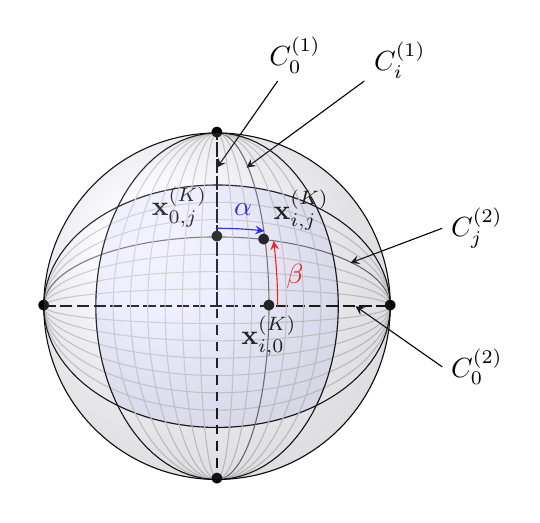
\begin{tikzpicture}[scale=2.2]
    \filldraw[draw=black,fill=blue!30!white,opacity=0.20]
	plot [smooth,domain=-35:35] ({0.7*cos(\x)},{sin(\x)})
	-- plot [smooth,domain=55:125] ({cos(\x)},{0.7*sin(\x)})
	-- plot [smooth,domain=140:215] ({0.7*cos(\x)},{sin(\x)})
	-- plot [smooth,domain=230:305] ({cos(\x)},{0.7*sin(\x)})
	-- cycle;	
	
	\draw [dashed, line width=0.8pt, samples=100,domain=180:-180] plot({cos(\x)},{0*sin(\x)});
	\draw [samples=100,domain=180:-180,color=gray!40] plot({cos(\x)},{0.1*sin(\x)});
	\draw [samples=100,domain=180:-180,color=gray!40] plot({cos(\x)},{0.2*sin(\x)});
	\draw [samples=100,domain=180:-180,color=gray!40] plot({cos(\x)},{0.3*sin(\x)});
	\draw [samples=100,domain=180:0,color=gray!120] plot({cos(\x)},{0.4*sin(\x)});
	\draw [samples=100,domain=0:-180,color=gray!40] plot({cos(\x)},{0.4*sin(\x)});
	\draw [samples=100,domain=180:-180,color=gray!40] plot({cos(\x)},{0.5*sin(\x)});
	\draw [samples=100,domain=180:-180,color=gray!40] plot({cos(\x)},{0.6*sin(\x)});
	\draw [samples=100,domain=180:-180] plot({cos(\x)},{0.7*sin(\x)});
	\draw [dashed, line width=0.8pt, samples=100,domain=180:-180] plot({0*cos(\x)},{sin(\x)});
	\draw [samples=100,domain=180:-180,color=gray!40] plot({0.1*cos(\x)},{sin(\x)});
	\draw [samples=100,domain=180:-180,color=gray!40] plot({0.2*cos(\x)},{sin(\x)});
	\draw [samples=100,domain=-90:90,color=gray!120] plot({0.3*cos(\x)},{sin(\x)});
	\draw [samples=100,domain=90:270,color=gray!40] plot({0.3*cos(\x)},{sin(\x)});
	\draw [samples=100,domain=180:-180,color=gray!40] plot({0.4*cos(\x)},{sin(\x)});
	\draw [samples=100,domain=180:-180,color=gray!40] plot({0.5*cos(\x)},{sin(\x)});
	\draw [samples=100,domain=180:-180,color=gray!40] plot({0.6*cos(\x)},{sin(\x)});
	\draw [samples=100,domain=180:-180] plot({0.7*cos(\x)},{sin(\x)}); 
	
	\draw [>=stealth, ->] (1.3,-.35) -- (.8,-0) ;
	\draw  (1.5,-.35) node {$C_0^{(2)}$} ;
	\draw [>=stealth, ->] (.35,1.3) -- (0,0.8) ;
	\draw  (.45,1.45) node {$C_0^{(1)}$} ;
	
	\draw [>=stealth, ->] (1.3,.45) -- (.77,0.25) ;
	\draw  (1.5,.45) node {$C_j^{(2)}$} ;
	
	\draw [>=stealth, ->] (.85,1.3) -- (.17,0.8) ;
	\draw  (.85,1.26) node[above right] {$C_i^{(1)}$} ;
	
	\draw  (0,1) node {$\bullet$} ;
	\draw  (0,-1) node {$\bullet$} ;
	\draw  (1,0) node {$\bullet$} ;
	\draw  (-1,0) node {$\bullet$} ;
	
	\draw  (.27,0.38) node {$\bullet$} ;
	\draw  (.27,0.38) node[above right] {$\mathbf{x}_{i,j}^{(K)}$} ;
	\draw  (0,0.4) node {$\bullet$} ;
	\draw  (0,0.4) node[above left] {$\mathbf{x}_{0,j}^{(K)}$} ;
	\draw  (0.3,0) node {$\bullet$} ;
	\draw  (.3,0) node[below] {$\mathbf{x}_{i,0}^{(K)}$} ;
	
	\draw [>=stealth, ->,samples=100,domain=90:75,color=blue] plot({1.05*cos(\x)},{0.45*sin(\x)});
	\draw  (.15,.65) node[color=blue, below] {$\alpha$} ;
	
	\draw [>=stealth, ->,samples=100,domain=0:21,color=red] plot({.35*cos(\x)},{1.05*sin(\x)});
	\draw  (.45,.3) node[color=red, below] {$\beta$} ;

	\draw (0,0) circle (1cm);
    \shade[ball color=blue!10!white,opacity=0.20] (0,0) circle (1cm);  
   
\end{tikzpicture}
\end{center}
\caption{Angles géodésiques $\alpha$ et $\beta$.}
\label{fig: alpha beta}
\end{figure}



\begin{figure}
\begin{center}
\begin{tikzpicture}[scale=2.5]
	\draw (1,3) -- (2,3) ; 
	\draw (0,2) -- (4,2) ; 	
	\draw (0,1) -- (4,1) ; 
	\draw (1,0) -- (2,0) ; 
	
	\draw (0,2) -- (0,1) ;
	\draw (1,3) -- (1,0) ;
	\draw (2,3) -- (2,0) ;
	\draw (3,2) -- (3,1) ;
	\draw (4,2) -- (4,1) ; 
	
	\draw [>=stealth, ->] (0.2,1.2) -- (0.5,1.2) ; 
	\draw (0.55,1.2) node[above]{$\alpha$} ; 
	\draw [>=stealth, ->] (0.2,1.2) -- (0.2,1.5) ; 
	\draw (0.3,1.4) node[above]{$\beta$} ; 
	\draw (0.7,1.7) node[above]{$(IV)$} ; 
	
	\draw [>=stealth, ->] (1.2,1.2) -- (1.5,1.2) ; 
	\draw (1.55,1.2) node[above]{$\alpha$} ; 
	\draw [>=stealth, ->] (1.2,1.2) -- (1.2,1.5) ; 
	\draw (1.3,1.4) node[above]{$\beta$} ; 
	\draw (1.7,1.7) node[above]{$(I)$} ; 
	
	\draw [>=stealth, ->] (2.2,1.2) -- (2.5,1.2) ; 
	\draw (2.55,1.2) node[above]{$\alpha$} ; 
	\draw [>=stealth, ->] (2.2,1.2) -- (2.2,1.5) ; 
	\draw (2.3,1.4) node[above]{$\beta$} ; 
	\draw (2.7,1.7) node[above]{$(II)$} ;
	
	\draw [>=stealth, ->] (3.2,1.2) -- (3.5,1.2) ; 
	\draw (3.55,1.2) node[above]{$\alpha$} ; 
	\draw [>=stealth, ->] (3.2,1.2) -- (3.2,1.5) ; 
	\draw (3.3,1.4) node[above]{$\beta$} ; 
	\draw (3.7,1.7) node[above]{$(III)$} ;  
	
	\draw [>=stealth, ->] (1.2,2.2) -- (1.5,2.2) ; 
	\draw (1.55,2.2) node[above]{$\alpha$} ; 
	\draw [>=stealth, ->] (1.2,2.2) -- (1.2,2.5) ; 
	\draw (1.3,2.4) node[above]{$\beta$} ; 
	\draw (1.7,2.7) node[above]{$(V)$} ; 
	
	\draw [>=stealth, ->] (1.2,0.2) -- (1.5,0.2) ; 
	\draw (1.55,0.2) node[above]{$\alpha$} ; 
	\draw [>=stealth, ->] (1.2,0.2) -- (1.2,0.5) ; 
	\draw (1.3,0.4) node[above]{$\beta$} ; 
	\draw (1.7,0.7) node[above]{$(VI)$} ; 
	
\end{tikzpicture}
\caption{Patron de la Cubed-Sphere avec orientation des directions $\alpha$ et $\beta$ par panel.}
\label{fig:patron cs}
\end{center}
\end{figure}

Si $\mathbf{x}_{i,j}^{(I)}$ un point du panel I de coordonnées $(x,y,z)$ dans $\mathbb{R}^3$. Alors les relations suivantes sont vérifiées :

\begin{equation}
\left\lbrace
\begin{array}{rcccc}
x & = & a \cos \alpha \cos \eta & = & a \cos \beta \cos \xi \\
y & = & a \sin \alpha & = & a \cos \beta \sin \xi \\
z & = & a \cos \alpha \sin \eta & = & a \sin \beta \\
\end{array}
\right.
\label{eq: panel I xyz xi eta alpha beta}
\end{equation}

Des relations similaires existent sur tous les panels (Voir tableau \ref{tab: x y z fct de xi eta alfa beta}).

\begin{table}[htbp]
\begin{center}
%\rotatebox{90}{
\begin{tabular}{|c|c|}
\hline
\textbf{Panel} & $(x,y,z)$ \textbf{fonction de} $(\alpha, \eta)$ \textbf{et de} $(\xi, \beta)$ \\

\hline
\hline
    & $x=a \cos \alpha \cos \eta  =  a \cos \beta \cos \xi$ \\ 
$I$ & $y=a \sin \alpha  =  a \cos \beta \sin \xi$ \\
    & $z=a \cos \alpha \sin \eta  =  a \sin \beta$ \\
\hline
\hline
      & $x=- a \sin \alpha  = - a \cos \beta \sin \xi$ \\ 
$II$  & $y=a \cos \alpha \cos \eta  =  a \cos \beta \cos \xi$ \\
      & $z=a \cos \alpha \sin \eta  =  a \sin \beta$ \\
\hline
\hline
      & $x=- a \cos \alpha \cos \eta = a \cos \beta \cos \xi$ \\ 
$III$ & $y=- a \sin \alpha = - a \cos \beta \sin \xi$ \\
      & $z=a \cos \alpha \sin \eta = a \sin \beta$ \\
\hline
\hline
      & $x=a \sin \alpha = a \cos \beta \sin \xi$ \\ 
$IV$  & $y=- a \cos \alpha \cos \eta = - a \cos \beta \cos \xi$ \\
      & $z=a \cos \alpha \sin \eta = a \sin \beta$ \\
\hline
\hline
    & $x=-a \cos \alpha \sin \eta = - a \sin \beta$ \\ 
$V$ & $y=a \sin \alpha = a \cos \beta \sin \xi$ \\
    & $z=a \cos \alpha \cos \eta = a \cos \beta \cos \xi$ \\
\hline
\hline
     & $x=a \cos \alpha \sin \eta = a \sin \beta$ \\ 
$VI$ & $y=a \sin \alpha = a \cos \beta \sin \xi$ \\
     & $z=- a \cos \alpha \cos \eta = - a \cos \beta \cos \xi$ \\
\hline
\end{tabular}
%}
\end{center}
\caption{$(x,y,z)$ fonction de $(\alpha, \eta)$ et de $(\xi, \beta)$  sur chaque panel.}
\label{tab: x y z fct de xi eta alfa beta}
\end{table}

Pour chaque panel, on peut déduire de \eqref{eq: panel I xyz xi eta alpha beta} les expressions de $\alpha$ et $\beta$ en fonction de $\xi$ et $\eta$. 

\begin{theoreme}
$(\alpha, \eta)$ et $(\xi, \beta)$ sont des systèmes de coordonnées admissibles par panel.
\end{theoreme} 

\begin{proof}
Conséquence des relations entre $(x,y,z)$ et $(\xi, \beta)$, $(\alpha, \eta)$ par panel (Voir tableau \ref{tab: x y z fct de xi eta alfa beta}).
\end{proof}


\begin{proposition}
$\alpha$ et $\beta$ s'expriment en fonction de $\xi$ et $\eta$ :

\begin{equation}
\left\lbrace
\begin{array}{rcl}
\alpha(\xi, \eta) & = & \arctan \left[ \dfrac{\tan \xi}{\sqrt{1+\tan^2 \eta}} \right] \\
\beta(\xi,\eta) & = & \arctan \left[ \dfrac{\tan \eta}{\sqrt{1+\tan^2 \xi}} \right] 
\end{array}
\right.
\label{eq: alpha et beta fct de xi et eta}
\end{equation}
\end{proposition}

\begin{proof}
Sur le panel I, $\alpha$ est une fonction construite sur un grand cercle, donc $\alpha$ sur le cercle constitué des points avec $\eta=\bar{\eta}$ constant. De même, $\beta$ varie avec $\xi= \bar{\xi}$ constant. 

On a :
\begin{equation}
x^2 + y^2 = a^2 \cos^2 \beta
\end{equation}
d'où on déduit facilement :
\begin{equation}
\tan^2 \beta = \dfrac{z^2}{x^2+y^2} = \dfrac{Y^2}{1+X^2}
\end{equation}
L'expression de $\beta$ suivante se déduit
\begin{equation}
\beta(\xi, \eta) = \arctan \left[ \dfrac{\tan \eta}{\sqrt{1+\tan^2 \xi}} \right]
\end{equation}
De la même manière on obtient :
\begin{equation}
\alpha(\xi, \eta) = \arctan \left[ \dfrac{\tan \xi}{\sqrt{1+\tan^2 \eta}} \right].
\end{equation}
De plus, ces équations se retrouvent sur chaque panel.
\end{proof}


\begin{theoreme}
$(\alpha, \beta)$ est un système de coordonnées admissible par panel.
\end{theoreme}

\begin{proof}

$\alpha$ et $\beta$ s'expriment en fonction de $X$ et $Y$ par :

\begin{equation}
\left\lbrace
\begin{array}{rcl}
\alpha & = & \arctan \left[ \dfrac{X}{\sqrt{1+ Y^2}} \right] \\
\beta & = & \arctan \left[ \dfrac{Y}{\sqrt{1+X^2}} \right] 
\end{array}
\right.
\label{eq: alpha et beta fct de X et Y}
\end{equation}

On pose $F : (X,Y) \mapsto (\alpha,  \beta)$, montrons que $F$ est bijective. La jacobienne de $F$ en $(X,Y)$, notée $J_{(X,Y)}F$, est :

\begin{equation}
J_{(X,Y)}F = \dfrac{1}{\delta^2} 
\begin{bmatrix}
\sqrt{1+Y^2} & - \dfrac{XY}{\sqrt{1+Y^2}} \\
- \dfrac{XY}{\sqrt{1+X^2}} & \sqrt{1+X^2}
\end{bmatrix}
\end{equation}

avec $\delta = \sqrt{1+X^2+Y^2}$. $F$ est bijective si $det \left( J_{(X,Y)}F \right) \neq 0$ pour tous $X,Y \in [-1,1]^2$.

\begin{equation}
det \left( J_{(X,Y)}F \right) = \dfrac{1}{\delta^2 \sqrt{(1+X^2)(1+Y^2)}} \neq 0
\end{equation}

donc $F$ est une bijection, $(X,Y)$ est un système de coordonnées admissible par panel donc $(\alpha, \beta)$ aussi.

\end{proof}























Chacune des portions de grands cercles peut être complétée en un grand cercle. Le grand cercle $C_i^{(1)}$ correspond à une isocline $\xi$ constante et le grand cercle $C_j^{(2)}$ à une isocline $\eta$ constante. Considérons l'isocline $\eta$ constante sur le panel I. Sur ce panel, l'angle $\alpha$ est tel que :

\begin{equation}
- \alpha_0 (\eta) \leq \alpha \leq \alpha_0(\eta) \text{ avec } \alpha_0( \eta) = \arctan \left( \dfrac{\sqrt{2}}{2} \tan \eta \right).
\end{equation}


Cependant le grand cercle $C_j^{(2)}$ passe aussi sur les panels II, III et IV dans cet ordre. On peut prolonger $\alpha$ comme étant l'angle curviligne le long du grand cercle complet. Sur le panel II, le grand cercle $C_j^{(2)}$ coupe d'autres grands cercles (ceux permettant de construire le panel II) en $\mathbf{M}_k$ ($-N/2 \leq k \leq N/2$) de coordonnées $(\xi^E_k = k \Delta \xi, \eta^E_k)$. Il coupe aussi le panel III mais correspond au points de maillage par symétrie, soit le grand cercle du panel III correspondant à l'isocline $\eta^B_k = \frac{\pi}{2} - \eta$. Enfin, le grand cercle $C_j^{(2)}$ intersecte le panel IV aux points de coordonnées $(\xi^W_k = k \Delta \xi, \eta^W_k)$. 

De la même manière, le grand cercle $C_i^{(1)}$ passe par les panels V, III et VI dans cet ordre et est paramétré par un angle $\beta$.

Les autres panels II, III, IV, V, VI sont traités de la même manière. Compte tenu des symétries de la Cubed-Sphere, 6 familles de grands cercles sont suffisantes. On définis les ensembles de grands cercles suivants :

\begin{itemize}
\item $(I_{\alpha})$ et $(I_{\beta})$ sont les grands cercles passant par le panel I. Ils sont définis comme les isolignes en $\eta$ et en $\xi$ (du panel I) respectivement,
\item $(II_{\alpha})$ et $(II_{\beta})$ sont les grands cercles passant par le panel II. Ils sont définis comme les isolignes en $\eta$ et en $\xi$ (du panel II) respectivement,
\item $(V_{\alpha})$ et $(V_{\beta})$ sont les grands cercles passant par le panel V. Ils sont définis comme les isolignes en $\eta$ et en $\xi$ (du panel V) respectivement.
\end{itemize}

\begin{figure}
\begin{center}
\includegraphics[scale=0.3]{fig21.jpg}
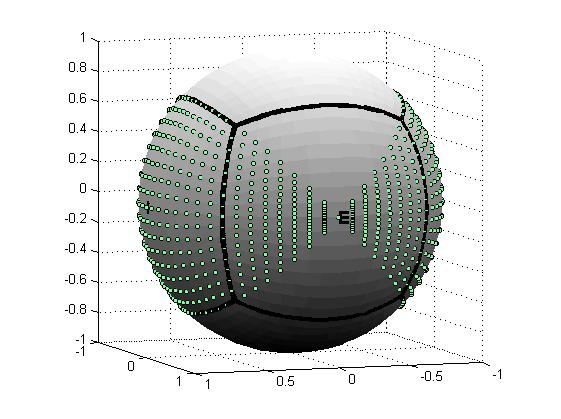
\includegraphics[scale=0.3]{fig22.jpg}
\end{center}
\caption{L'ensemble $(I_{\alpha})$ de grands cercles correspond aux isoclines $\eta$ constant du panel I et du panel III.}
\end{figure}


La structure de la Cubed-Sphere issus de grands cercles est la base du procédé de calcul de dérivées hermitiennes que nous utilisons dans ce travail. Le calcul du gradient suis la procédure suivante :

\begin{enumerate}
\item Construction de données le long de grands cercles complets,
\item Calcul des dérivées hermitiennes,
\item Assemblage pour obtenir le gradient.
\end{enumerate}




Pour calculer $\dfrac{\partial h}{\partial \alpha}_{|C_1}$ et $\dfrac{\partial h}{\partial \beta}_{|C_2}$ aux points de maillage, il sera utile de connaître les coordonnées des points d'intersections de grands cercles entre les panels.

Soit $h_{i,j}^k$ donné avec $-N/2 \leq i,j \leq N/2$ et $k = I, II, III, IV, V, VI$. Considérons le grand cercle $C_1 \in (I_{\alpha})$. Il correspond à l'isocline $\eta = \eta_0^F = j_0 \Delta \eta$. Les valeurs $h_{i,j_0}^F$ sont localisée sur un grand cercle avec $-N/2 \leq i \leq N/2$. En continuant sur le cercle $C_1$, on traverse le panel II sur lequel il faudra interpoler les données pour compléter les valeurs le long de $C_1$. Le cercle $C_1$ coupe chaque isocline $\xi = \xi^E_{i_0} = i_0 \Delta \xi$ au point de coordonnées $(\xi_{i_0}^E, \beta_{i_0,j_0})$ dans le système de coordonnées $(\xi^E, \beta)$ du panel II. Un point $(x,y,z)\in \mathbb{R}^3$ d'un cercle de $(II_{\beta})$ est donné par :

\begin{equation}
\left\lbrace
\begin{array}{rcl}
x & = & - a \cos \beta \sin \xi^E \\
y & = & a \cos \beta \cos \xi^E \\
z & = & a \sin \beta
\end{array}
\right.
\end{equation}

Le point $\mathbf{x}(x,y,z)$ est se situe à l'intersection de $C_1$ (isocline $\eta^F_{j_0}$ du panel I) avec le grand cercle correspondant à l'isocline $\xi = \xi^E_{i_0} = i_0 \Delta \xi$ si $x$, $y$ et $z$ sont solutions du système suivant :

\begin{equation}
\left\lbrace
\begin{array}{rcccl}
x & = & a \cos \alpha_{i_0, j_0} \cos \eta^F_{j_0} & = & a \cos \beta_{i_0, j_0} \cos \xi^E_{i_0} \\
y & = & a \sin \alpha_{i_0, j_0} & = & a \cos \beta_{i_0, j_0} \cos \xi^E_{i_0} \\
z & = & a \cos \alpha_{i_0, j_0} \sin \eta^F_{j_0}  & = & a \sin \beta_{i_0, j_0}
\end{array}
\right.
\end{equation}

de là, il découle :

\begin{equation}
\dfrac{z}{x} = \tan \eta^F_{j_0} = - \dfrac{\sin \beta_{i_0, j_0}}{\cos \beta_{i_0, j_0} \sin \xi^E_{i_0}}
\end{equation}

donc :

\begin{equation}
\beta_{i_0, j_0} = \arctan \left[ - \tan \eta^F_{j_0} \sin \xi^E_{i_0} \right]
\end{equation}

Ainsi, le point du panel II de coordonnées $(\xi, \beta)$, représentant l'intersection de l'isocline $\eta^F_{j_0}$ du panel I avec l'isocline $\xi_{i_0}^E$ du panel II, est donné par $(\xi^E_{i_0}, \beta_{i_0, j_0})$. En général, il ne s'agit pas d'un point de la Cubed-Sphere. Nous utiliserons une méthode de spline cubique pour obtenir des valeurs $u_{i_0,j}^{II}$ le long de $C$.
En continuant ce procédé, nous obtenons des valeurs tout du long du cercle $C$.







On peut calculer les dérivées partielles $\dfrac{\partial h}{\partial \alpha}_{|C_1}$ et $\dfrac{\partial h}{\partial \beta}_{|C_2}$ en fonction des paramètres $\xi$ et $\eta$. Par composition, les relations suivantes sont vérifiées :

\begin{equation}
\begin{array}{rcl}
\dfrac{\partial h}{\partial \alpha}_{|C_1} & = &  \dfrac{1}{\frac{\partial \alpha}{\partial \xi}} \dfrac{\partial h}{\partial \xi}_{|C_1} \\
\dfrac{\partial h}{\partial \beta}_{|C_2} & = &  \dfrac{1}{\frac{\partial \beta}{\partial \eta}} \dfrac{\partial h}{\partial \eta}_{|C_2} \\
\end{array}
\label{eq: derivee partiel link}
\end{equation}






On peut calculer les vecteurs $\mathbf{g}_{\alpha}$, $\mathbf{g}_{\beta}$, $\mathbf{g}^{\alpha}$ et $\mathbf{g}^{\beta}$. Par commodité, on écrira ces vecteurs en fonction de $\mathbf{g}_{\xi}$, $\mathbf{g}_{\eta}$, $\mathbf{g}^{\xi}$ et $\mathbf{g}^{\eta}$ :

\begin{proposition}
Les expressions suivantes sont vérifiées :
\begin{itemize}
\item $\mathbf{e}_{\alpha} = \dfrac{1}{\frac{\partial \alpha}{\partial \xi}} \mathbf{g}_{\xi}$,
\item $\mathbf{e}_{\beta} = \dfrac{1}{\frac{\partial \beta}{\partial \eta}} \mathbf{g}_{\eta}$,
\item $\mathbf{e}^{\alpha} = \dfrac{\partial \alpha}{\partial \xi} \mathbf{g}^{\xi}$,
\item $\mathbf{e}^{\beta} = \dfrac{\partial \beta}{\partial \eta} \mathbf{g}^{\eta}$.
\end{itemize}
\label{prop: g_alpha g_beta fct de g_xi g_eta}
\end{proposition}

\begin{proof}
\begin{itemize}
\item Par définition et composition, on a :

\begin{equation}
\mathbf{g}_{\xi} = \dfrac{d \mathbf{x}}{d \xi} = \dfrac{\partial \alpha}{\partial \xi} \dfrac{d \mathbf{x}}{d \alpha} = \dfrac{\partial \alpha}{\partial \xi} \mathbf{e}_{\alpha}.
\end{equation}

d'où le premier résultat :

\begin{equation}
\mathbf{e}_{\alpha} = \dfrac{1}{\frac{\partial \alpha}{\partial \xi}} \mathbf{g}_{\xi}
\end{equation}

De la même manière :

\begin{equation}
\mathbf{e}_{\beta} = \dfrac{1}{\frac{\partial \beta}{\partial \eta}} \mathbf{g}_{\eta}
\end{equation}

\item On pose $\mathbf{u} = \dfrac{\partial \alpha}{\partial \xi} \mathbf{g}^{\xi}$ et $\mathbf{v} = \dfrac{\partial \beta}{\partial \eta} \mathbf{g}^{\eta}$. Alors :

\begin{equation}
\mathbf{e}_{\alpha} \cdot \mathbf{u} = \dfrac{\frac{\partial \alpha}{\partial \xi}}{\frac{\partial \alpha}{\partial \xi}} \mathbf{g}_{\xi} \cdot \mathbf{g}^{\xi} = 1.
\end{equation}

De plus :

\begin{equation}
\mathbf{e}_{\beta} \cdot \mathbf{u} = \dfrac{\frac{\partial \alpha}{\partial \xi}}{\frac{\partial \beta}{\partial \eta}} \mathbf{g}_{\eta} \cdot \mathbf{g}^{\xi} = 0
\end{equation}

Donc $\mathbf{e}^{\alpha} = \mathbf{u}$. De la même manière, on montre que $\mathbf{e}^{\beta} = \mathbf{v}$.
\end{itemize}
\end{proof}




\begin{theoreme}
Si $h : \mathbb{S}_a^2 \rightarrow \mathbb{R}$ est une fonction régulière, alors :
\begin{equation}
\nabla_T h = \dfrac{\partial h}{\partial \xi}_{|\eta = \bar{\eta}} \mathbf{g}^{\xi} + \dfrac{\partial h}{\partial \eta}_{|\xi = \bar{\xi}} \mathbf{g}^{\eta}
\end{equation}
\label{th:gradient_xieta}
\end{theoreme}


\begin{proof}
Les égalités suivantes est vérifiées grâce à la proposition \ref{prop: g_alpha g_beta fct de g_xi g_eta} et aux équations \eqref{eq: derivee partiel link} :

\begin{equation}
\dfrac{\partial h}{\partial \alpha}_{|C_1} \mathbf{e}^{\alpha} = \dfrac{1}{\alpha'(\xi)} \dfrac{\partial h}{\partial \xi}_{|\eta = \bar{\eta}} \alpha'(\xi) \mathbf{g}^{\xi} = \dfrac{\partial h}{\partial \xi}_{|\eta = \bar{\eta}} \mathbf{g}^{\xi}
\end{equation}

De même :

\begin{equation}
\dfrac{\partial h}{\partial \beta}_{|C_2} \mathbf{e}^{\beta} =  \dfrac{\partial h}{\partial \eta}_{|\xi = \bar{\xi}} \mathbf{g}^{\eta}
\end{equation}

d'où le résultat immédiat à l'aide de la formule \eqref{eq: gradient}.
\end{proof}









